\documentclass[12pt,twoside,abbrevs,msc,ai,notimes,logo,sansheadings]{infthesis}

% Packages
\usepackage{graphicx}
\usepackage{abbrevs}
\usepackage{acronym}
% Will use listings instead for now. minted isn't included in the ubuntu texlive version. \usepackage{minted}
\usepackage{multirow}

% Added packages
\usepackage{cite}
\usepackage{listings}
\usepackage{hyperref} % for \url
\usepackage{amstext} % for \text
\usepackage{subcaption} % for \subfloat
\usepackage{epstopdf} % for eps images
% \usepackage{beramono} % for bera mono font

% only needed for \usepackage{fancyvrb}. \renewcommand\theFancyVerbLine{\normalsize\arabic{FancyVerbLine}}

% Added config
\setlength{\parskip}{0pt plus12pt minus4pt}
\raggedbottom

% Project Details
\title{Parallelising Plan Recognition}
\author{Chris Swetenham}
\course{MSc Artificial Intelligence}
\project{Dissertation}

\submityear{2012}
\graduationdate{November 2012}
\date{\today}

% TODO other acronyms
\newacro{CAS}{Compare And Swap}
\newacro{CCG}{Combinatory Categorial Grammar}

\abstract{

Plan Recognition is an area of Artificial Intelligence research with many potential applications in which it is desirable to perform it in real time. In order to devise a performant solution for plan recognition, we study the ELEXIR algorithm for plan recognition in C++. We find it well suited to parallelisation using multithreaded job scheduling techniques and apply several scheduling techniques, including lock-free work stealing. We and analyse and report on the speed and scalability of these techniques when applied to plan recognition.
}


% Extra Package Commands

\begin{document}
  \begin{preliminary}
    % Title Page
    \maketitle

    % Preamble
    \begin{acknowledgements}

	Thanks to my supervisor, Chris Geib, for his support during this project.

\end{acknowledgements}

    \standarddeclaration
    %\dedication{

TODO is this even included

}
 TODO?
    \tableofcontents
    \listoffigures
  \end{preliminary}

% Sides per Section (Planned)
% ---------------------------
% Title page 1
% Blank 1
% Abstract 1
% Acknowledgements 1
% Declaration 1
% Blank 1
% TOC 2
% List of Figures 1
% Blank 1
% Intro 1
% Blank 1
% Background 8
% Related Work 1
% Blank 1
% Initial Work 3
% Blank 1
% Method 0 1
% Blank 1
% Method 1 2
% Method 2 3
% Blank 1
% Method 3 4
% Method 4 2
% Analysis 3
% Blank 1
% Conclusion 1
% Bibliography 2
% --------------
% Total 47

  
  % Chapters
  % Introduction: background to the project, previous work, exposition of relevant literature, setting of the work in the proper context.
  \chapter{Introduction}

Plan Recognition is a problem which consists of looking at a sequence of actions by an agent, and deduce possible goals that these actions achieve. Plan Recognition has many potential applications, including network intrusion detection, human-robot interaction and assisted care scenarios.

In many of these potential problem domains, including the ones mentioned above, it is desirable to perform plan recognition in real time, rather than offline as a batch computation. However currently, for performance reasons, it is often infeasible to perform Plan Recognition in real time.

In this project, we investigate several methods for parallelising a particular Plan Recognition algorithm in C++. We investigate the performance on two different problem domains, and how the performance scales up with the number of available hardware threads.


  \chapter{Background}

TODO

\section{Plan Recognition}

TODO discuss plan recognition and its potential applications
TODO discuss plan recog is symbolic, how it fits into larger system (e.g. get symbols from behaviour recog, get grammars authored or learned (future work))

\section{Combinatorial Categorical Grammars}

TODO describe Categorical Grammars, Combinatorial Categorical Grammars

\section{Applying CCGs to Plan Recognition}

TODO

\section{The ELEXIR Algorithm}

TODO describe the ELEXIR algorithm

\section{Concurrency Techniques}

TODO describe locking and lock-free techniques
TODO describe mutexes, condition variables
TODO describe memory barriers, atomic operations, hazard pointers (or later?)
TODO describe performance issues: waiting, kernel switches, busy waits, starvation, priority inversion, cache contention and false sharing
TODO describe correctness issues: missed wake-ups, deadlocks, static/dynamic hazards, ABA problem, ...

\section{Multicore Job Scheduling Techniques}

TODO describe single queue
TODO describe multiple queues with main thread redistributing work
TODO describe work-stealing
TODO reference that XB360/dev conf talk on job queues?
TODO mention dependencies between tasks, tasks producing other tasks

\section{Applying Job Scheduling Techniques to ELEXIR}

TODO describe how ELEXIR is well-suited to job scheduling - tasks generate the new tasks that depend on them, pure fan-out with no dependencies sideways and no shared resources needing to be updated
TODO describe how we choose to split work
TODO Work out the complexity (Could go in appendix)

TODO Work out the perfect $T_1$ to $T_\infty$ speedup (Could go in appendix)

  \chapter{Related Work}

We now look at some related efforts in terms of Plan Recognition and parallelisation. Various Approaches to probabilistic Plan Recognition based on Hidden Markov Models (HMMs) and Conditional Random Fields (CRFs) exist. The AHMM model\cite{bib:hmm} allows online, probabilistic Plan Recognition, including a representation of the state of the world and its effect on the planning of agents; however, it does not deal with interleaved or partially-ordered plans.
Graph-based methods reduce plan recognition to a graph covering problem. The algorithm in \cite{bib:graph} is able to perform Plan Recognition lazily, computing explanations efficiently and only as needed, but it does not provide probabilities for the explanations, and does not deal with interleaved or partially-ordered plans.

There is extensive literature on parallelising search problems\cite{bib:search}, and some of this could be applicable to Plan Recognition algorithms. However, since ELEXIR performs an exhaustive rather than heuristic search, they are not directly applicable to this project. There has been some work on parallelising the parsing problem\cite{bib:parsing}, however this applies mainly to traditional parsing problems based on context-free grammars with no ambiguity, where only a single parse will result from a given input. These methods do not need to deal with contextual effects and multiple parse explanations. They are applicable to much larger inputs presented in batch form, such as program source millions of lines long. Parallelisation strategies are therefore quite different from the ones we consider, for example by starting simultaneous parses at multiple points in the input stream and combining the resulting partial parse trees.

Clark and Curran have developed a parallel implementation for learning of CCGs in Natural Language\cite{bib:ccgpar}, which runs in parallel and distributed fashion on a Beowulf cluster. However, the parsing aspect is not a complete parallel parser like the one we develop here.

The influential Cilk algorithm\cite{bib:workstealing} schedules strict computations with dependencies between tasks. This paper discusses the advantages of work-stealing over work-sharing algorithms, and gives bounds on the efficiency of work-stealing. Chase \& Lev describe an algorithm\cite{bib:queue} for a lock-free work-stealing queue, which we base ourselves on for our own implementation.

  % Description of the work undertaken: this may be divided into chapters describing the conceptual design work and the actual implementation separately. Any problems or difficulties and the suggested solutions should be mentioned. Alternative solutions and their evaluation should be included.
  \chapter{Initial Work}
  Before starting with the implementation of multithreading, we evaluated the existing ELEXIR codebase to detect any potential issues. We used the \emph{Memcheck} tool within the \emph{Valgrind} program on Linux to detect memory leaks which we then fixed. Valgrind dynamically translates the machine code being executed and allows its tools to insert instrumentation before the code is actually executed. Memcheck tracks memory allocations and can warn of both memory leaks and invalid memory accesses.
  
  The reference-counting was changed to use reference-counting smart pointers rather than the manual incrementing and decrementing initially present. This helped fix a number of memory leaks. It was also modified to use atomic incrementing and decrementing of reference counts, and this was sufficient to ensure thread safety, since threads incrementing the reference count always own at least one reference to it through the explanation currently being processed. In order to verify that the changes made to the code did not break existing functionality, we added tests for the results of the algorithm on one of the domains. We also added unit tests for some of the new functionality.
  
  We considered several possible libraries for implementing multithreading. We chose the \emph{Boost Threads} library, which is part of the \emph{Boost} project, over the POSIX threading API for reasons of both convenience and portability; although the code has not yet been ported entirely to Windows, the added code was designed with this future port in mind.
  
  The executable compiled for evaluation runs takes as parameters the domain and problem files to be processed. In addition, command-line arguments allow specifying the number of explanations to allocate in each task, and the maximum number of worker threads to spawn. Except in Method 1, it will never spawn more worker threads than there are hardware threads available.
  
  The code for this project was developed using Boost version 1.46.1 on Ubuntu Linux 12.04 64-bit, and also tested and run using Boost version 1.41 on Scientific Linux 6.2. The machines used for evaluation are Sherlock, a 4-core Intel i5 desktop PC with 8GB of memory running the Ubuntu configuration, and Catzilla, a 16-core AMD Opteron multi-user server with 64GB of memory running the Scientific Linux configuration.
  
  Boost 1.46.1 is the currently packaged version of Boost on Ubuntu 12.04. Unfortunately it suffers from an occasional deadlock issue due to locking order when a sleeping thread is interrupted by calling boost::thread::interrupt(). We encountered this issue during development which for certain build configurations and datasets would very reliably cause deadlocks. Interruption was being used to exit threads when processing was complete. Interruption causes an exception to be thrown in the interrupted thread; we replaced calls to thread::interrupt() with a task that throws this exception when invoked. The entry function of the worker thread then catches this exception and exits the thread.
  
  Each algorithm is implemented with a similar structure: a class encapsulates the algorithm, and is instantiated based on the selected algorithm for each run. This class has a method which is called on the main thread, and creates the worker threads. Each of the threads runs a static method on the class, which interacts with a \texttt{WorkerData} structure containing the queues or other relevant information. The worker thread method is mostly independent of the nature of the work being done. Finally, tasks are represented by a \texttt{TaskData} structure which contains the expressions for the task, and any other relevant data. This structure has a method which is passed a pointer to the \texttt{WorkerData}, processes the expressions, and passes the results back into new tasks or to the main thread.
  
  The two problem domains used for evaluation are the XPERIENCE domain, which involves hands picking up and moving balls around and into cups, and is based on the XPERIENCE robotics project [TODO: cite]; and the Logistics domain, which involves trucks and airplanes transporting packages between cities, and is based on the Logistics domain in the First International Planning Competition [TODO: cite].
  
  \chapter {Method 0 - Original Single-Threaded ELEXIR}
  
  The first method we include for comparison is a mostly unmodified single-threaded implementation.
  
  \section {Implementation}
  
  On each new observation, the entire current list of explanations is looped over by the main thread, and a new list of explanations is generated. The batch size and thread count parameters are ignored.
  
  [TODO: code snippet]
  
  \section{Evaluation}
  
  Since this method does not scale with the number of threads, we will report baseline performance numbers, shown in Table~\ref{tab:m0}.
  
  \begin{table}
  \begin{tabular}{c c c}
  Domain & Sherlock Runtime (seconds) & Catzilla Runtime (seconds)\tabularnewline
  \hline
  XPERIENCE Domain & 5.63 & 14.67\tabularnewline
  Logistics Domain & 1.36 & TODO\tabularnewline
  \hline
  \end{tabular}
  \caption{Average Runtimes for Method 0}
  \label{tab:m0}
  \end{table}

  \chapter {Method 1 - One Thread Per Task}
  
  As a proof of concept for multithreading the algorithm, this method spawns a new thread for each task, one task per hardware thread up to the thread limit.
  
  \section {Implementation}
  
  On each new observation,  the main thread spawns a new thread for each task, equal to the number of hardware threads available or the thread limit. Each task processes its explanations and produces new resulting explanations. The main thread waits for all the spawned threads to complete, and collects their results, then spawns a new set of threads on the next observation. This implementation ignores the batch size parameter and partitions the explanations evenly between tasks.
  
  [TODO: code snippet]
  
  \section{Evaluation}
  
  \begin{figure}[!htbp]
  \centering{}
  \begin{minipage}[t]{0.49\columnwidth}
  \subfloat[Runtime]{
    \begin{centering}
    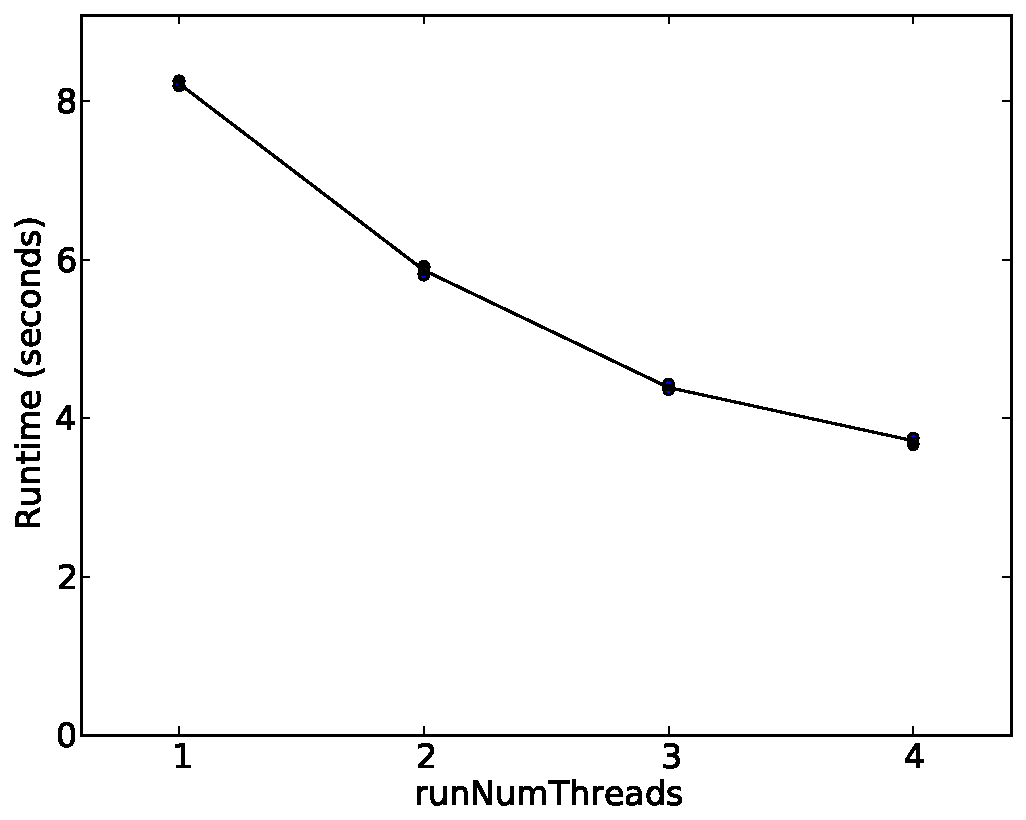
\includegraphics[scale=0.40]{{{images/threads-xper5-sherlock-1-1}}}
    \end{centering}
  }
  \end{minipage}
  \begin{minipage}[t]{0.49\columnwidth}
  \subfloat[Throughput]{
    \begin{centering}
    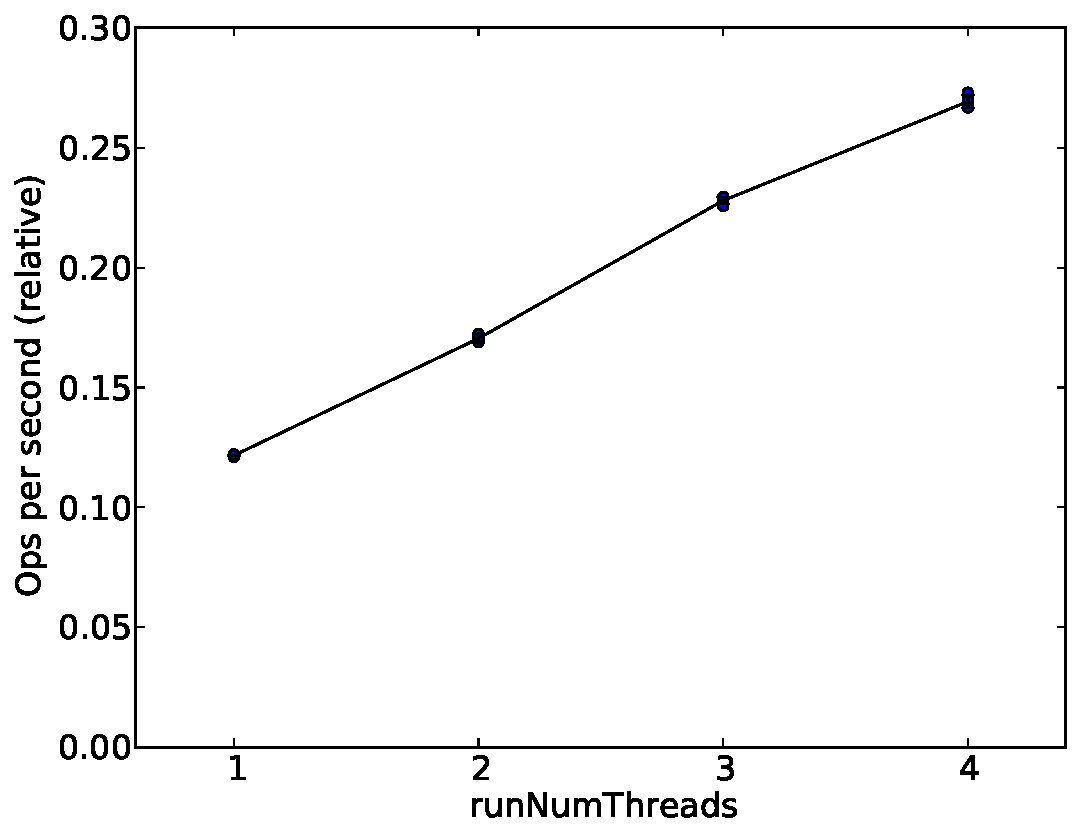
\includegraphics[scale=0.40]{{{images/threads-xper5-sherlock-1-2}}}
    \end{centering}
  }
  \end{minipage}
  \caption{Runtime with 1 to 4 threads on Sherlock, Method 1, XPERIENCE domain}
  \label{fig:thread-s1x}
  \end{figure}
  
  \begin{figure}[!htbp]
  \centering{}
  \begin{minipage}[t]{0.49\columnwidth}
  \subfloat[Runtime]{
    \begin{centering}
    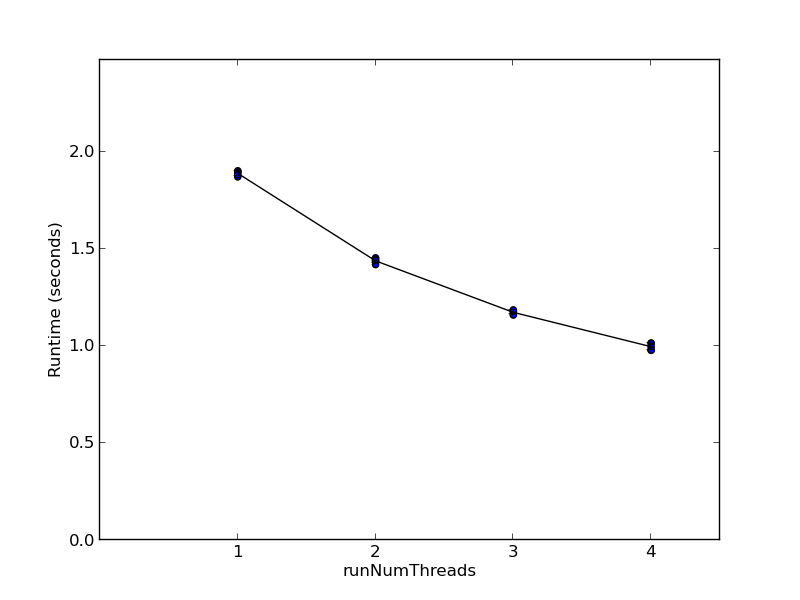
\includegraphics[scale=0.40]{{{images/threads-log3-sherlock-1-1}}}
    \end{centering}
  }
  \end{minipage}
  \begin{minipage}[t]{0.49\columnwidth}
  \subfloat[Throughput]{
    \begin{centering}
    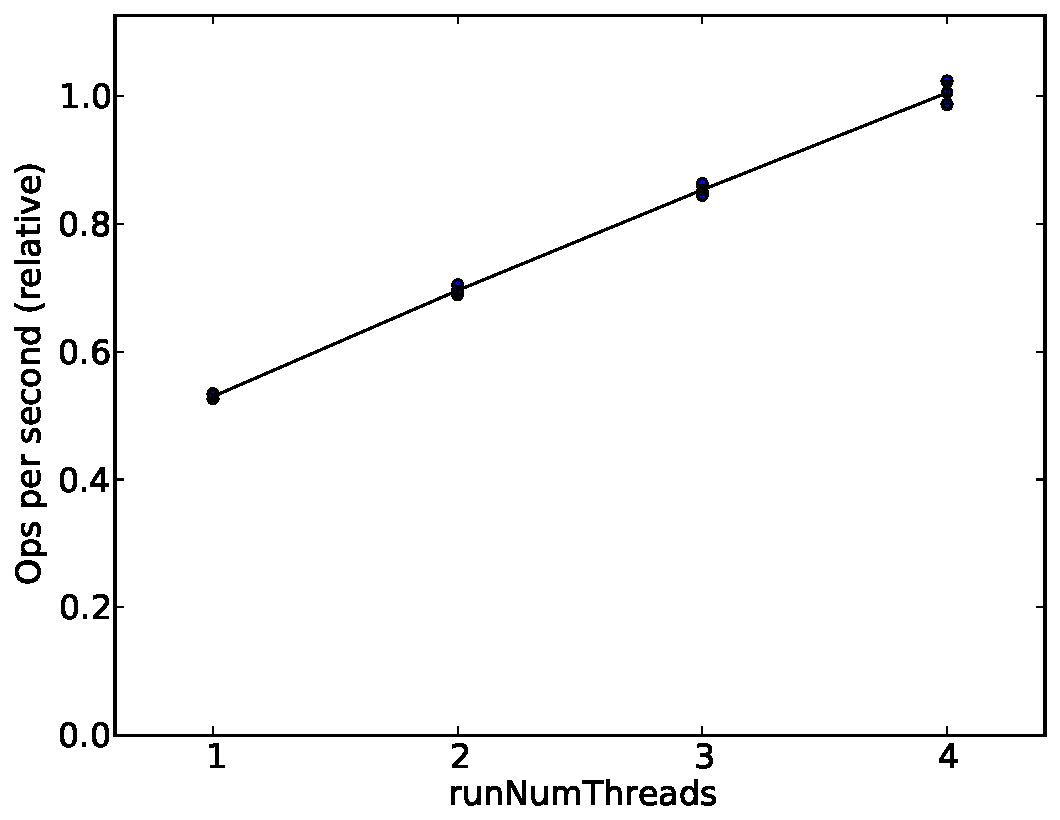
\includegraphics[scale=0.40]{{{images/threads-log3-sherlock-1-2}}}
    \end{centering}
  }
  \end{minipage}
  \caption{Runtime with 1 to 4 threads on Sherlock, Method 1, Logistics domain}
  \label{fig:thread-s1l}
  \end{figure}
  
  \begin{figure}[!htbp]
  \centering{}
  \begin{minipage}[t]{0.49\columnwidth}
  \subfloat[Runtime]{
    \begin{centering}
    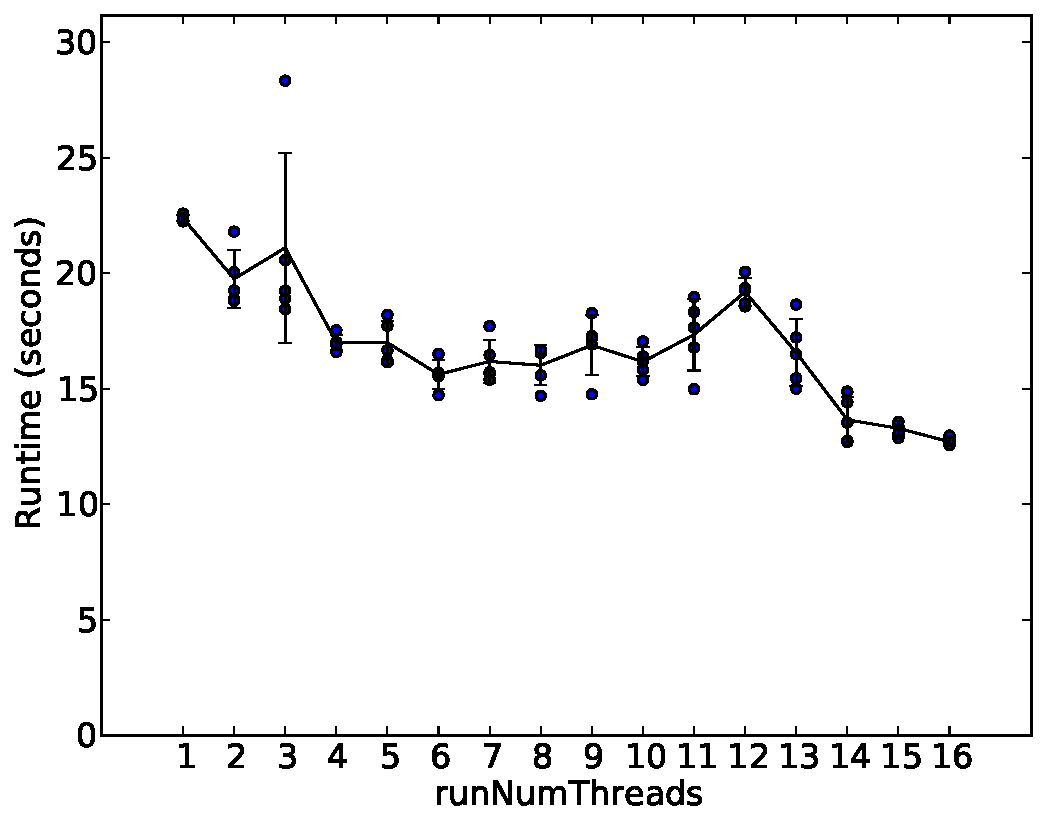
\includegraphics[scale=0.40]{{{images/threads-xper5-catzilla.inf.ed.ac.uk-1-1}}}
    \end{centering}
  }
  \end{minipage}
  \begin{minipage}[t]{0.49\columnwidth}
  \subfloat[Throughput]{
    \begin{centering}
    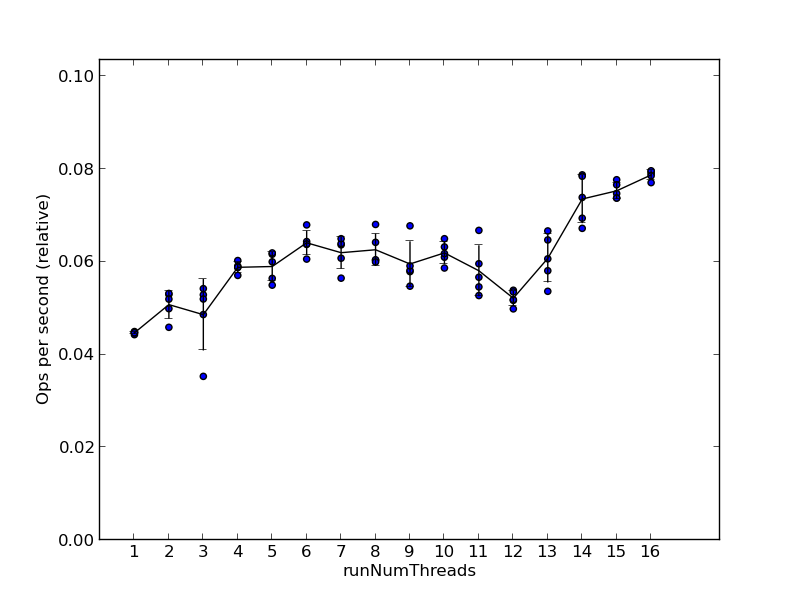
\includegraphics[scale=0.40]{{{images/threads-xper5-catzilla.inf.ed.ac.uk-1-2}}}
    \end{centering}
  }
  \end{minipage}
  \caption{Runtime with 1 to 16 threads on Catzilla, Method 1, XPERIENCE domain}
  \label{fig:thread-c1x}
  \end{figure}
  
  \begin{figure}[!htbp]
  \centering{}
  \begin{minipage}[t]{0.49\columnwidth}
  \subfloat[Runtime]{
    \begin{centering}
    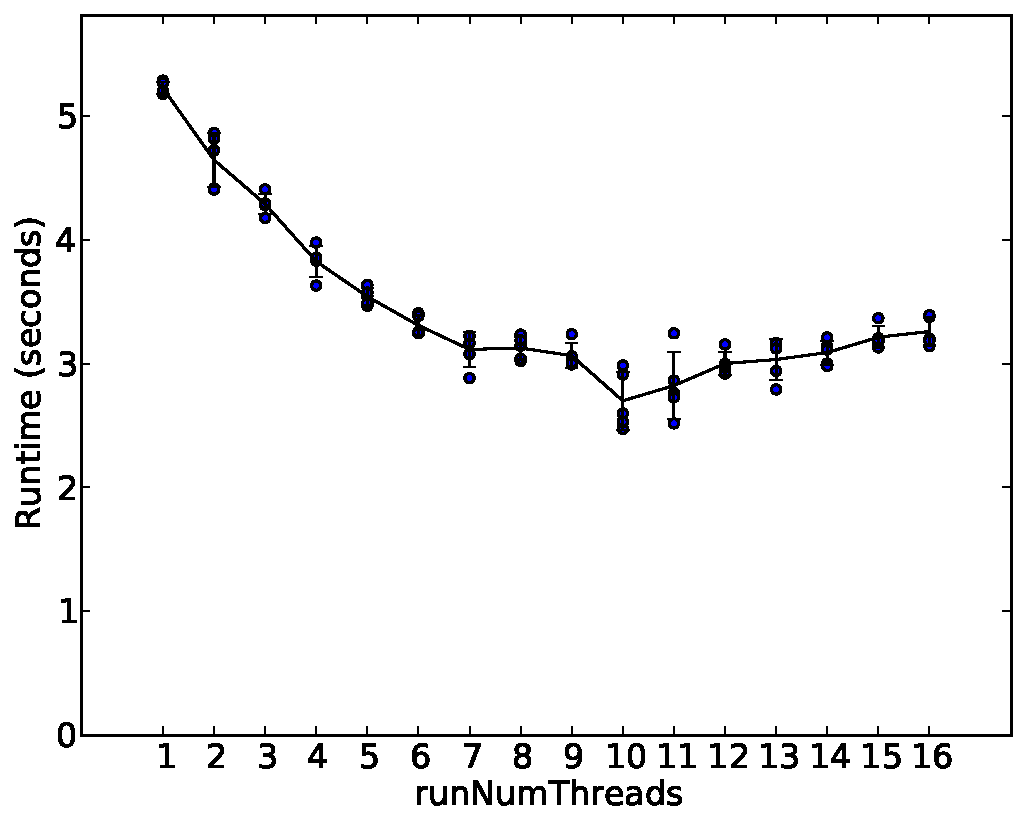
\includegraphics[scale=0.40]{{{images/threads-log3-catzilla.inf.ed.ac.uk-1-1}}}
    \end{centering}
  }
  \end{minipage}
  \begin{minipage}[t]{0.49\columnwidth}
  \subfloat[Throughput]{
    \begin{centering}
    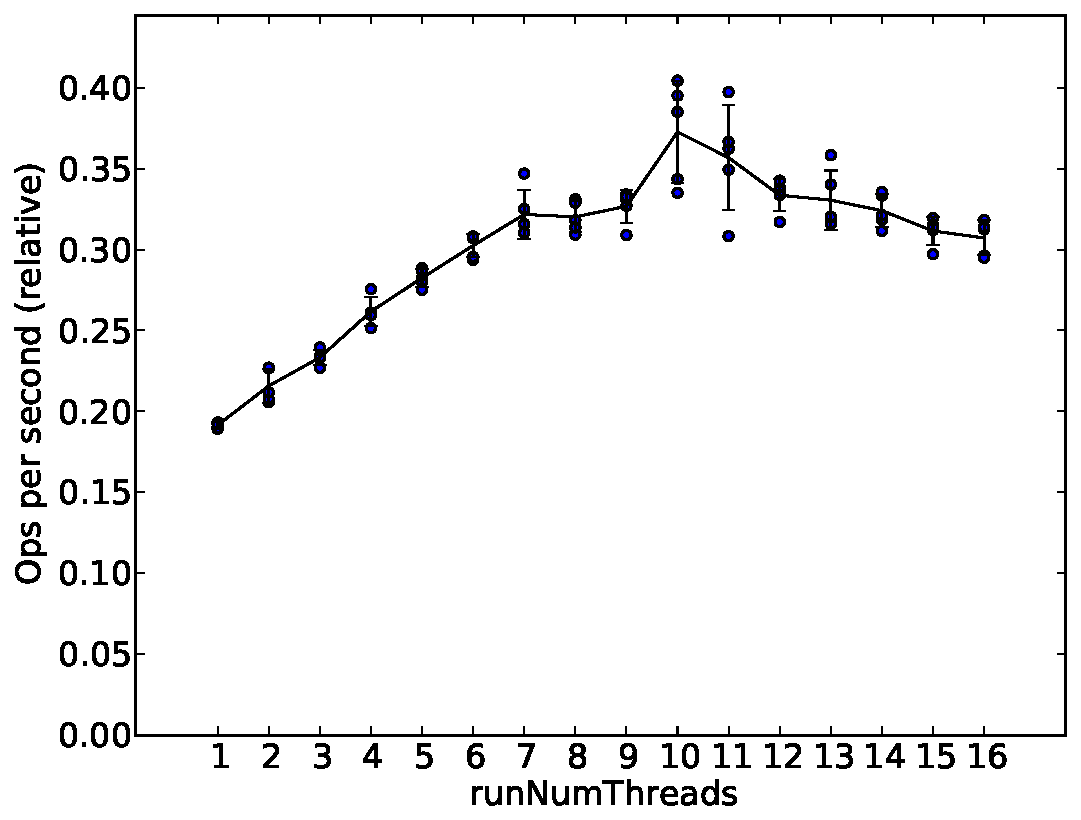
\includegraphics[scale=0.40]{{{images/threads-log3-catzilla.inf.ed.ac.uk-1-2}}}
    \end{centering}
  }
  \end{minipage}
  \caption{Runtime with 1 to 16 threads on Catzilla, Method 1, Logistics domain}
  \label{fig:thread-c1l}
  \end{figure}
  
  \chapter {Method 2 - One Queue Per Thread}
  
  This method uses one blocking queue per thread, guarded by a mutual exclusion lock.
  
  \section {Implementation}
  
  The main thread creates a queue for each worker thread, then spawns the threads. On each new observation, the main thread partitions the work evenly between the worker thread queues, and waits for them to finish processing them, finally collecting the new explanations.
  
  The implementation of the queue is based on boost::bounded\_buffer from the documentation of the Boost Circular Buffer library. Internally, it uses a bounded circular buffer guarded by a mutex. Worker threads trying to fetch work wait on a condition variable which is signalled when work is added to the buffer. The main difference between this method and the previous one is that the threads sleep between observations rather than exiting and being recreated.
  
  Completion is detected using a completion barrier as described in The Art of Multiprocessor Programming [TODO: cite]. A count of active threads is maintained and atomically incremented and decremented by worker threads as they become busy or idle.
  
  This implementation does not take into account the batch size parameter, since the main thread is responsible for redistributing the work. The main thread creates as task for each worker thread and splits the explanation to be processed evenly between them.
  
  \section{Evaluation}
  
  \begin{figure}[!htbp]
  \centering{}
  \begin{minipage}[t]{0.49\columnwidth}
  \subfloat[Runtime]{
    \begin{centering}
    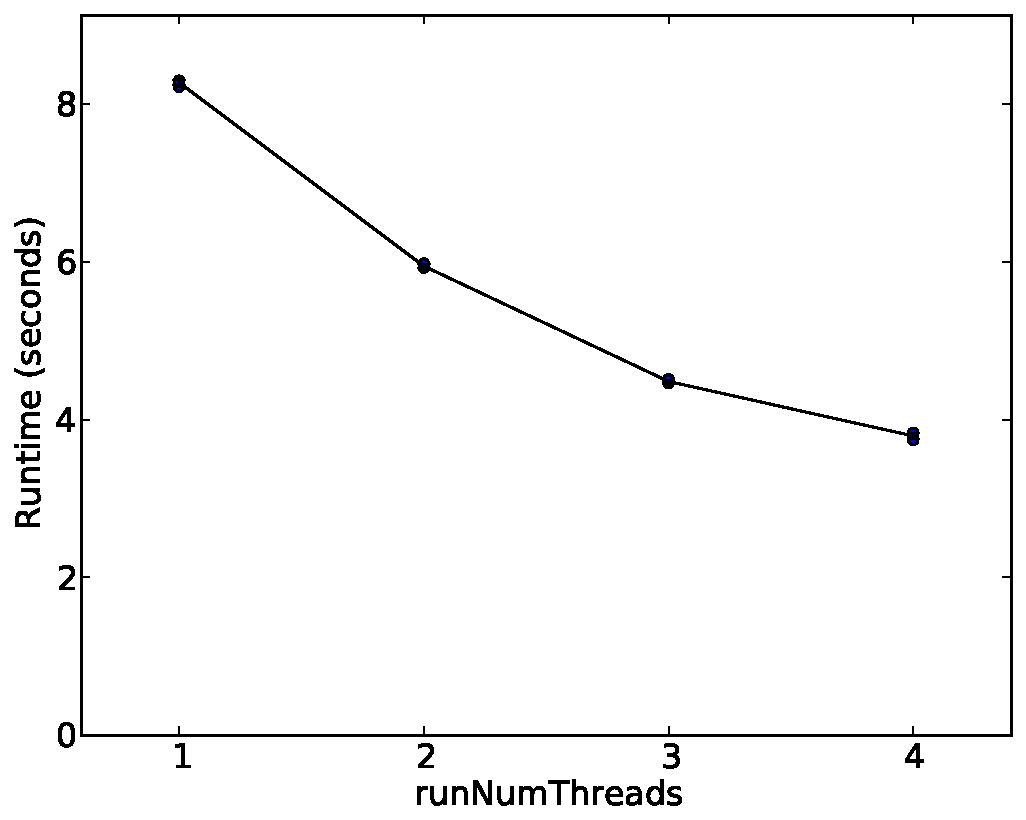
\includegraphics[scale=0.40]{{{images/threads-xper5-sherlock-2-1}}}
    \end{centering}
  }
  \end{minipage}
  \begin{minipage}[t]{0.49\columnwidth}
  \subfloat[Throughput]{
    \begin{centering}
    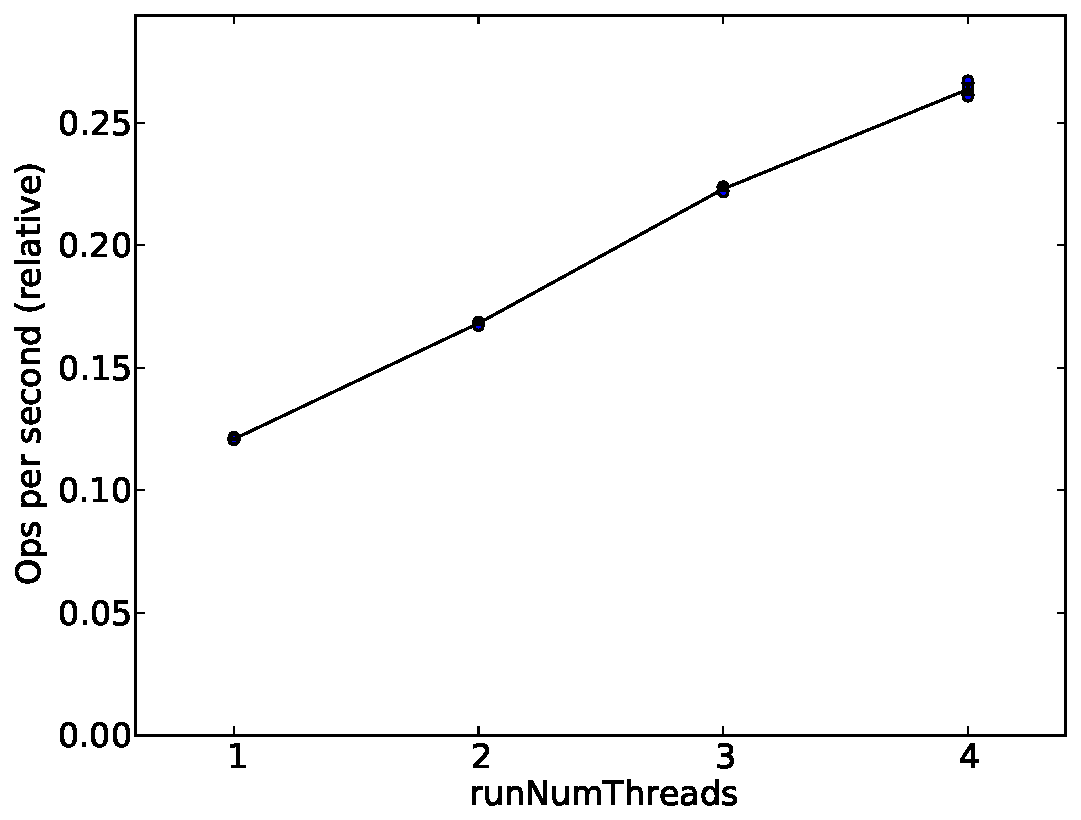
\includegraphics[scale=0.40]{{{images/threads-xper5-sherlock-2-2}}}
    \end{centering}
  }
  \end{minipage}
  \caption{Runtime with 1 to 4 threads on Sherlock, Method 2, XPERIENCE domain}
  \label{fig:thread-s2x}
  \end{figure}
  
  \begin{figure}[!htbp]
  \centering{}
  \begin{minipage}[t]{0.49\columnwidth}
  \subfloat[Runtime]{
    \begin{centering}
    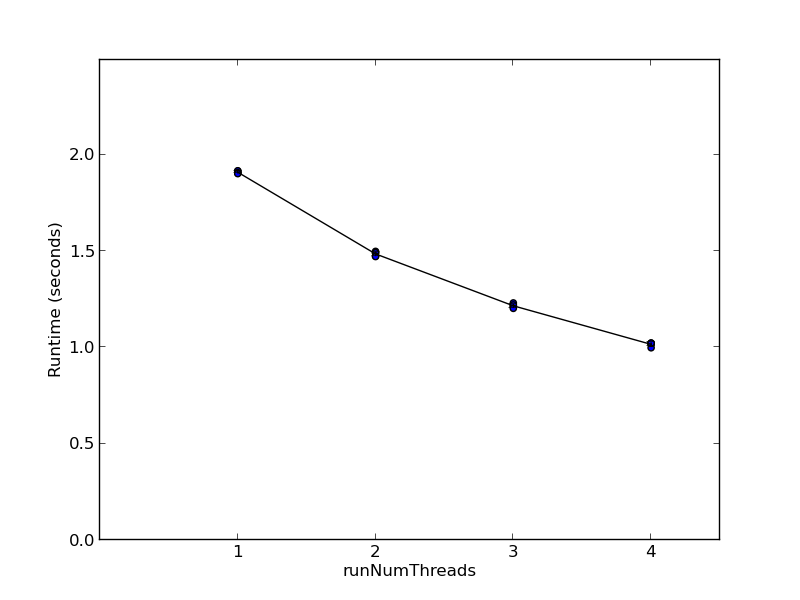
\includegraphics[scale=0.40]{{{images/threads-log3-sherlock-2-1}}}
    \end{centering}
  }
  \end{minipage}
  \begin{minipage}[t]{0.49\columnwidth}
  \subfloat[Throughput]{
    \begin{centering}
    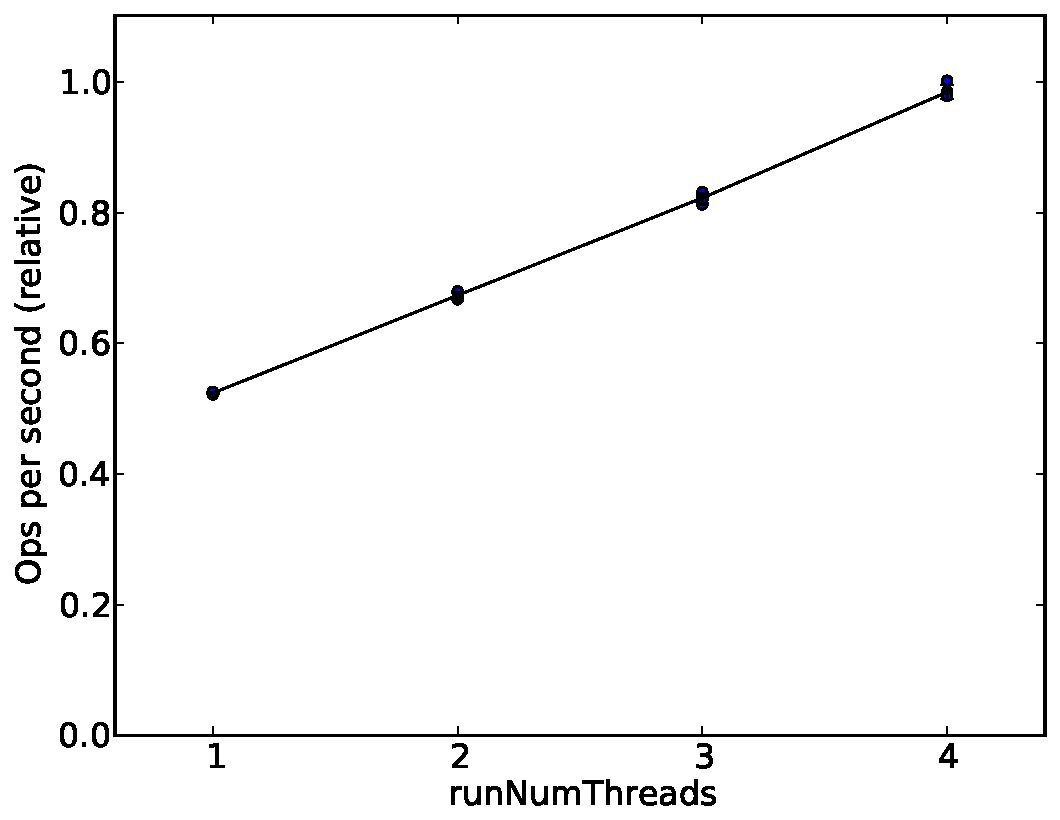
\includegraphics[scale=0.40]{{{images/threads-log3-sherlock-2-2}}}
    \end{centering}
  }
  \end{minipage}
  \caption{Runtime with 1 to 4 threads on Sherlock, Method 2, Logistics domain}
  \label{fig:thread-s2l}
  \end{figure}
  
  \begin{figure}[!htbp]
  \centering{}
  \begin{minipage}[t]{0.49\columnwidth}
  \subfloat[Runtime]{
    \begin{centering}
    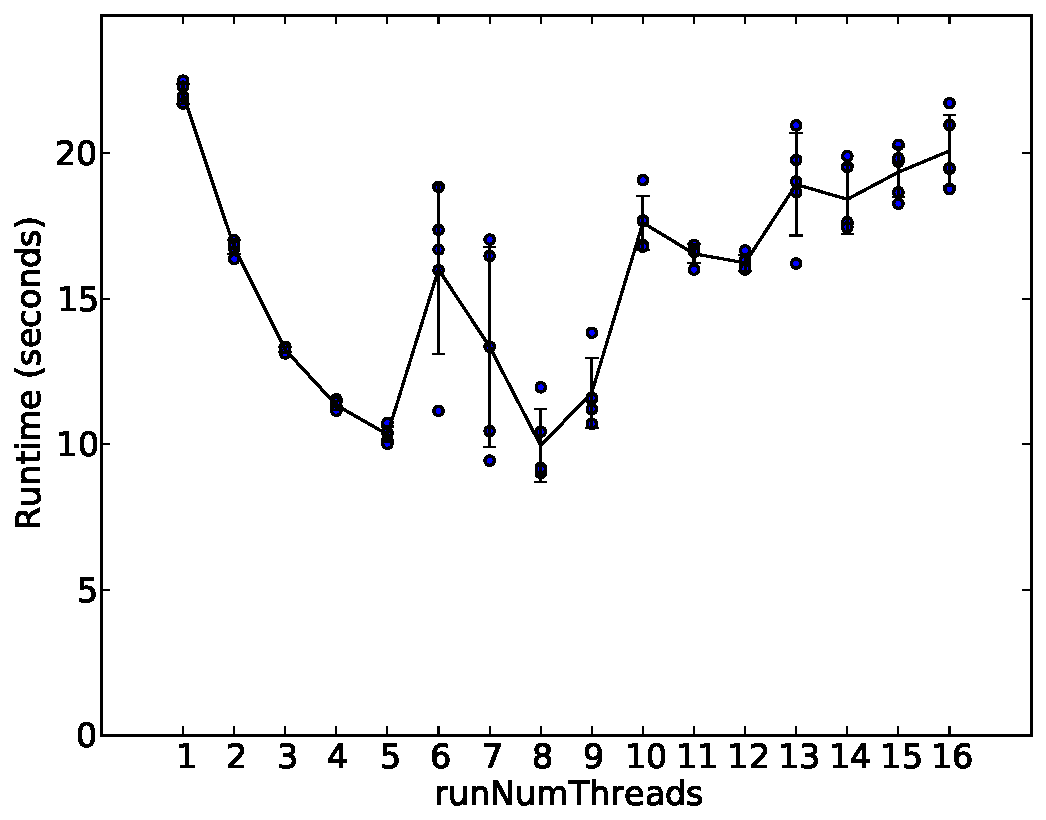
\includegraphics[scale=0.40]{{{images/threads-xper5-catzilla.inf.ed.ac.uk-2-1}}}
    \end{centering}
  }
  \end{minipage}
  \begin{minipage}[t]{0.49\columnwidth}
  \subfloat[Throughput]{
    \begin{centering}
    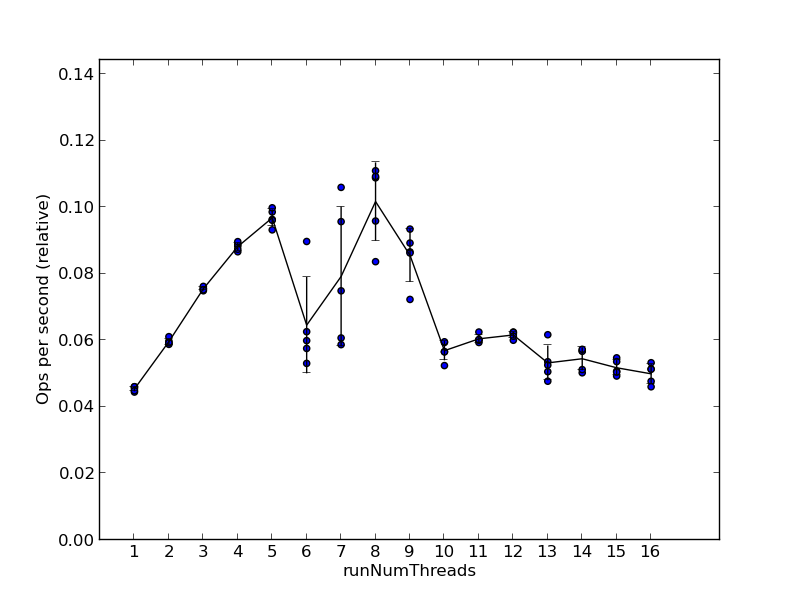
\includegraphics[scale=0.40]{{{images/threads-xper5-catzilla.inf.ed.ac.uk-2-2}}}
    \end{centering}
  }
  \end{minipage}
  \caption{Runtime with 1 to 16 threads on Catzilla, Method 1, XPERIENCE domain}
  \label{fig:thread-c2x}
  \end{figure}
  
  \begin{figure}[!htbp]
  \centering{}
  \begin{minipage}[t]{0.49\columnwidth}
  \subfloat[Runtime]{
    \begin{centering}
    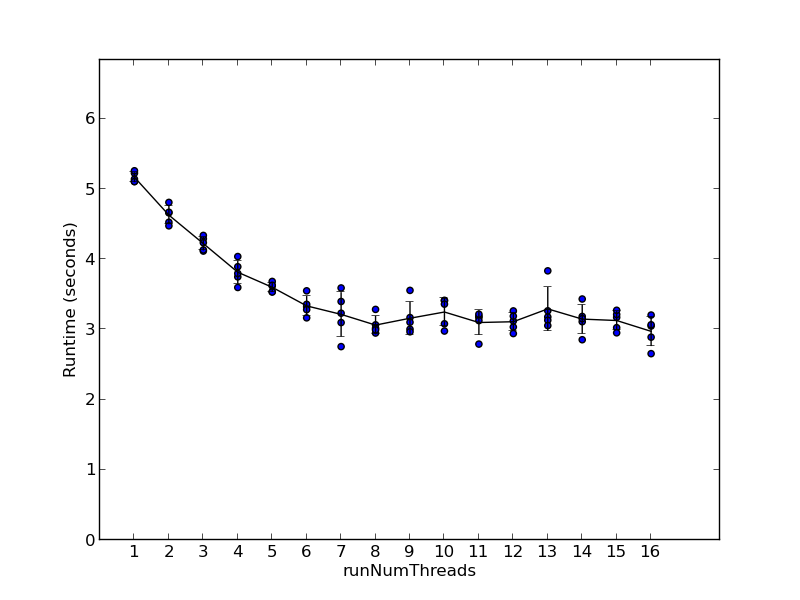
\includegraphics[scale=0.40]{{{images/threads-log3-catzilla.inf.ed.ac.uk-2-1}}}
    \end{centering}
  }
  \end{minipage}
  \begin{minipage}[t]{0.49\columnwidth}
  \subfloat[Throughput]{
    \begin{centering}
    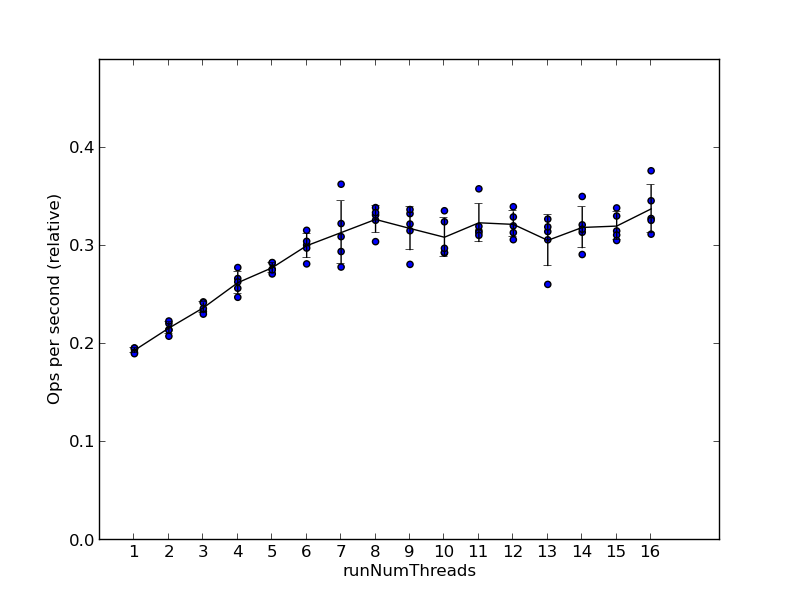
\includegraphics[scale=0.40]{{{images/threads-log3-catzilla.inf.ed.ac.uk-2-2}}}
    \end{centering}
  }
  \end{minipage}
  \caption{Runtime with 1 to 16 threads on Catzilla, Method 2, Logistics domain}
  \label{fig:thread-c2l}
  \end{figure}
  
  \section{Analysis}
  TODO
  
  \chapter {Method 3 - Lock-Free Work-Stealing}
  
  This method uses one lock-free queue for each worker thread. Other threads can steal from this queue if they run out of work in their own queue.
  
  \section {Implementation}
  
  The implementation of this scheduler is based on [TODO: cite], also described in The Art of Multiprocessor Programming [TODO: cite], which describes a lock-free work-stealing queue where stealing threads steal a single task from the tail of the victim thread's queue, and threads otherwise insert and retrieve work from the head of their own queue. The queue can be resized safely if there is not enough space to insert work at the head of the queue. The original implementation described is appropriate for the language Java where memory is managed by garbage collection, and reads and writes to volatile variables are not reordered. In order to implement this in C++, the replacement of the queue's buffer when it is reallocated had to be guarded using \emph{hazard pointers} [TODO: cite] and the ordering of reads and writes to variables accessed locklessly enforced using compiler-specific memory fence directives. [TODO: cite gcc manual? Or footnote + cite]
  
  In terms of performance, we expect this implementation to have low contention due to the lack of locking, and good load-balancing since idle threads will steal work from other threads. During initial testing, we found that performance would drop as the number of threads increased from 2 to 4 threads. Using cachegrind to produce a differential profile between a run with 1 thread and a run with 4 threads, we discovered that idle threads were spending a lot of time in random number generation, which is used when selecting a victim thread to steal from. The insertion of a short sleep after failed stealing attempts resolved this issue.
   
  [TODO: code snippet]
  
  \section{Evaluation}
  
  \subsection{Batch Size Parameter}
  
  In order to estimate the best value for the batch size parameter, we ran the implementation with 4 threads on the XPERIENCE domain, varying the batch size.
  
  \begin{figure}[!htbp]
  \begin{centering}
  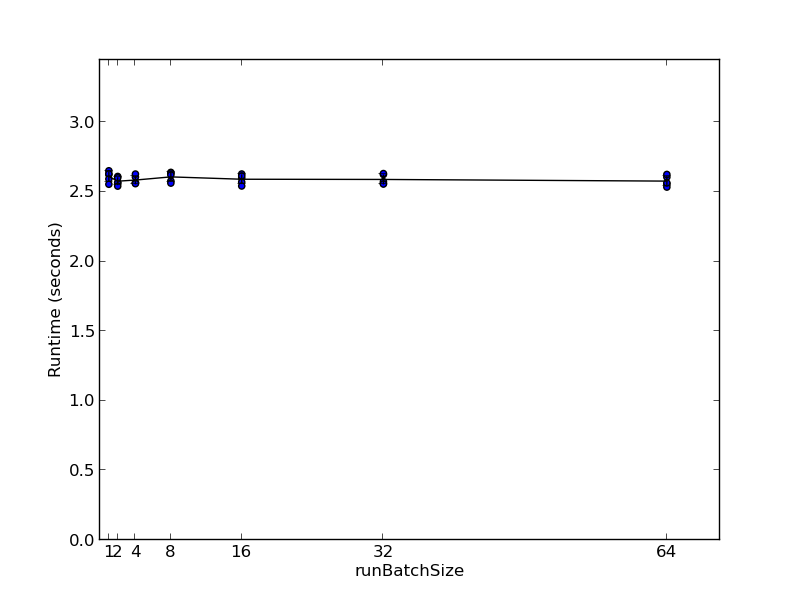
\includegraphics[width=0.8\textwidth]{{{images/batch-xper5-sherlock-3-1}}}
  \par\end{centering}
  \caption{Runtime with varying batch size on Sherlock, Method 3, XPERIENCE domain}
  \label{fig:batch-3}
  \end{figure}
  
  We can see in Figure~\ref{fig:batch-3} that the batch size does not significantly affect the runtime for this algorithm. All further tests were performed with a batch size of 8.
  
  \subsection{Thread Count}
  \begin{figure}[!htbp]
  \centering{}
  \begin{minipage}[t]{0.49\columnwidth}
  \subfloat[Runtime]{
    \begin{centering}
    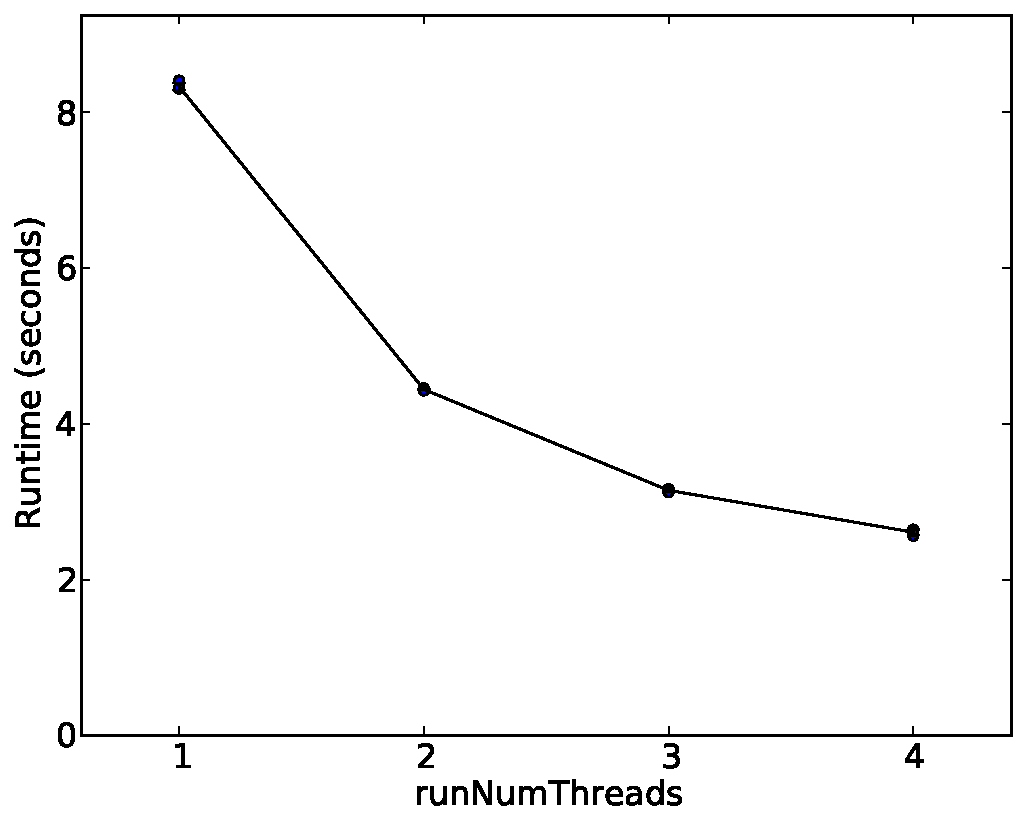
\includegraphics[scale=0.40]{{{images/threads-xper5-sherlock-3-1}}}
    \end{centering}
  }
  \end{minipage}
  \begin{minipage}[t]{0.49\columnwidth}
  \subfloat[Throughput]{
    \begin{centering}
    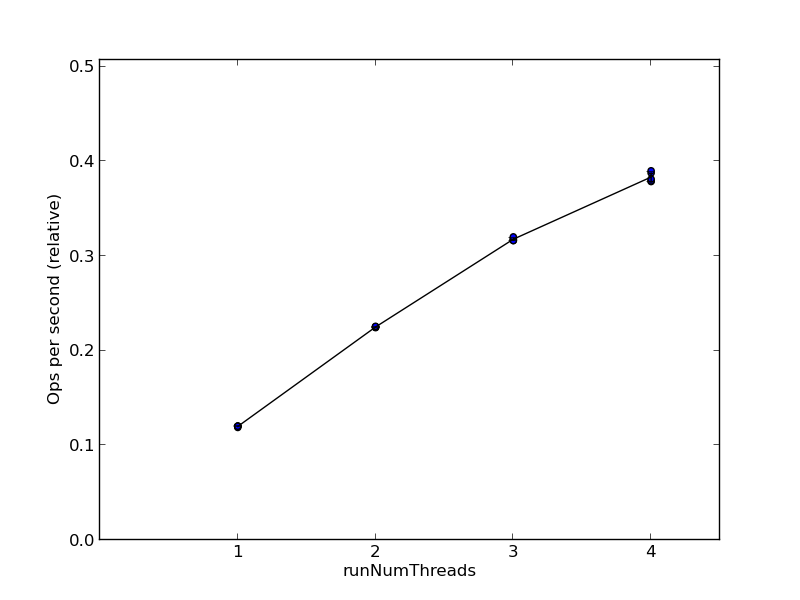
\includegraphics[scale=0.40]{{{images/threads-xper5-sherlock-3-2}}}
    \end{centering}
  }
  \end{minipage}
  \caption{Runtime with 1 to 4 threads on Sherlock, Method 3, XPERIENCE domain}
  \label{fig:thread-s3x}
  \end{figure}
  
  \begin{figure}[!htbp]
  \centering{}
  \begin{minipage}[t]{0.49\columnwidth}
  \subfloat[Runtime]{
    \begin{centering}
    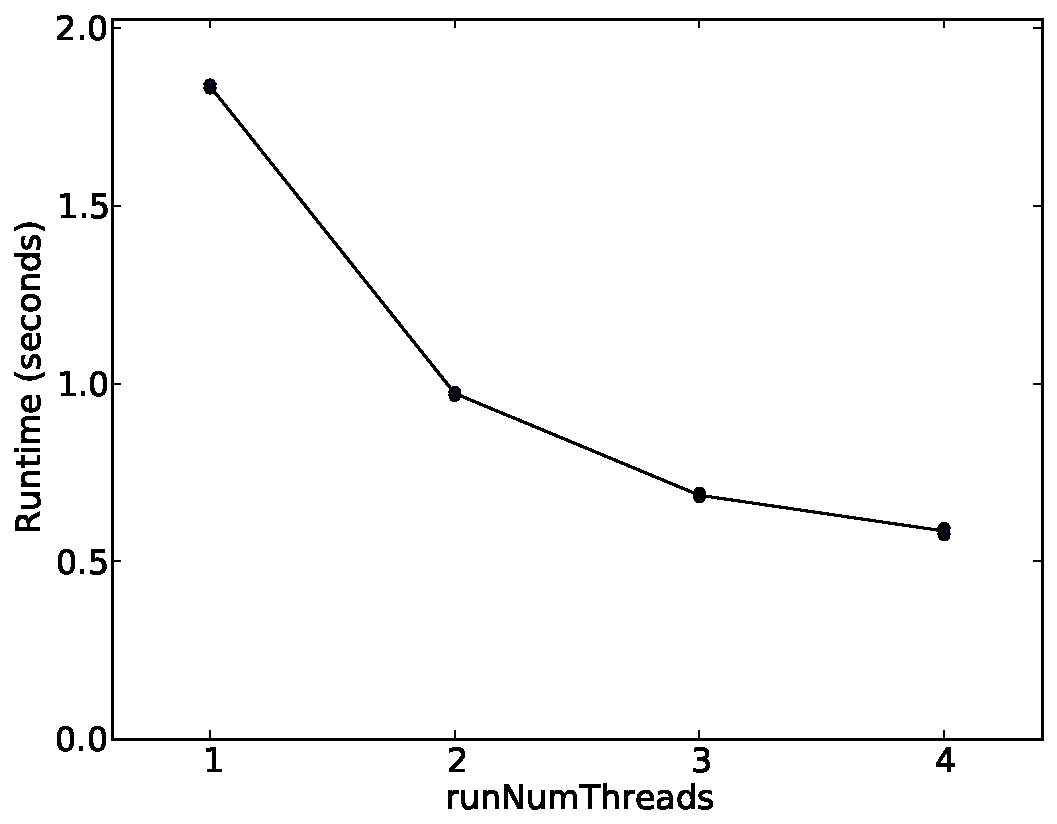
\includegraphics[scale=0.40]{{{images/threads-log3-sherlock-3-1}}}
    \end{centering}
  }
  \end{minipage}
  \begin{minipage}[t]{0.49\columnwidth}
  \subfloat[Throughput]{
    \begin{centering}
    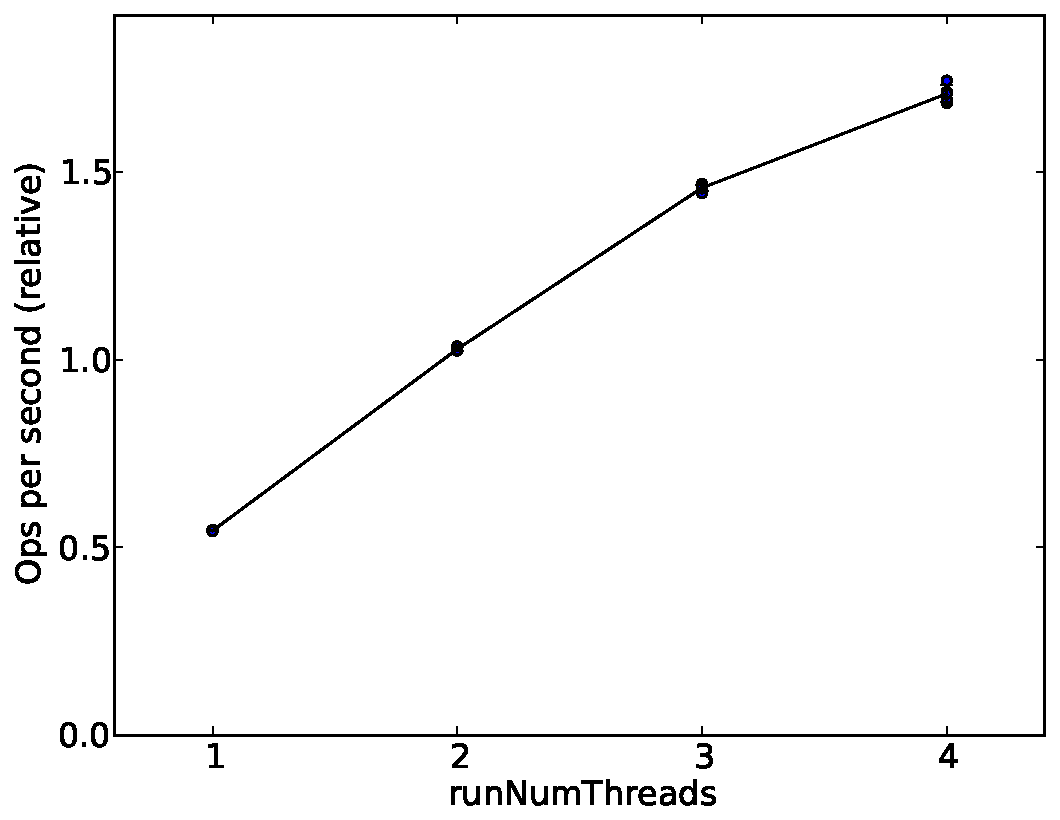
\includegraphics[scale=0.40]{{{images/threads-log3-sherlock-3-2}}}
    \end{centering}
  }
  \end{minipage}
  \caption{Runtime with 1 to 4 threads on Sherlock, Method 3, Logistics domain}
  \label{fig:thread-s3l}
  \end{figure}
  
  \begin{figure}[!htbp]
  \centering{}
  \begin{minipage}[t]{0.49\columnwidth}
  \subfloat[Runtime]{
    \begin{centering}
    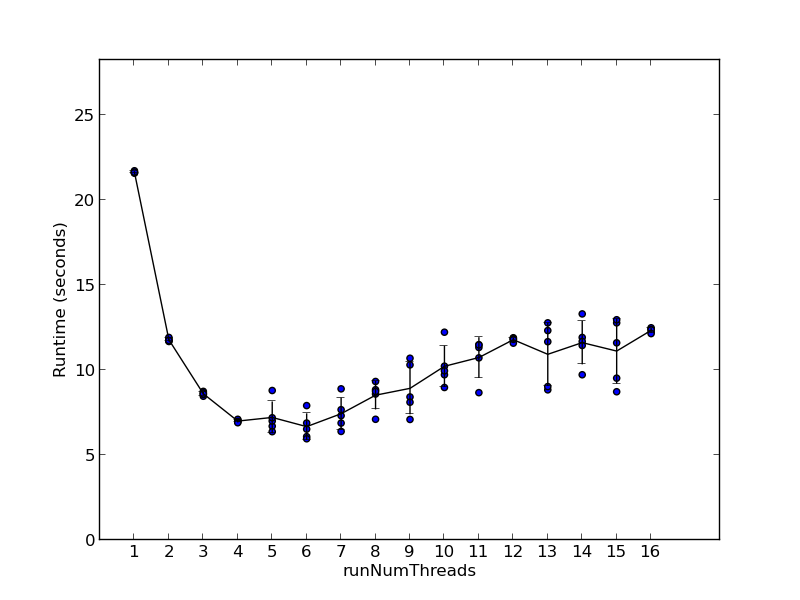
\includegraphics[scale=0.40]{{{images/threads-xper5-catzilla.inf.ed.ac.uk-3-1}}}
    \end{centering}
  }
  \end{minipage}
  \begin{minipage}[t]{0.49\columnwidth}
  \subfloat[Throughput]{
    \begin{centering}
    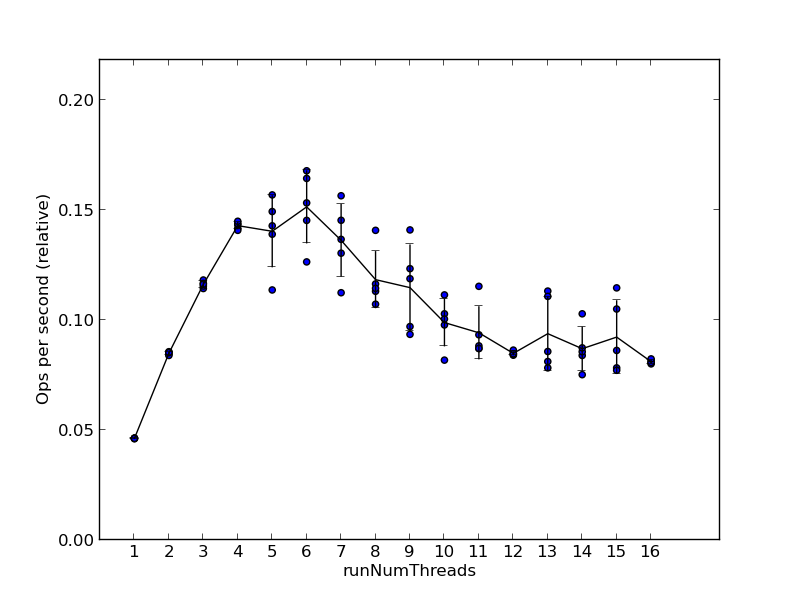
\includegraphics[scale=0.40]{{{images/threads-xper5-catzilla.inf.ed.ac.uk-3-2}}}
    \end{centering}
  }
  \end{minipage}
  \caption{Runtime with 1 to 16 threads on Catzilla, Method 3, XPERIENCE domain}
  \label{fig:thread-c3x}
  \end{figure}
  
  \begin{figure}[!htbp]
  \centering{}
  \begin{minipage}[t]{0.49\columnwidth}
  \subfloat[Runtime]{
    \begin{centering}
    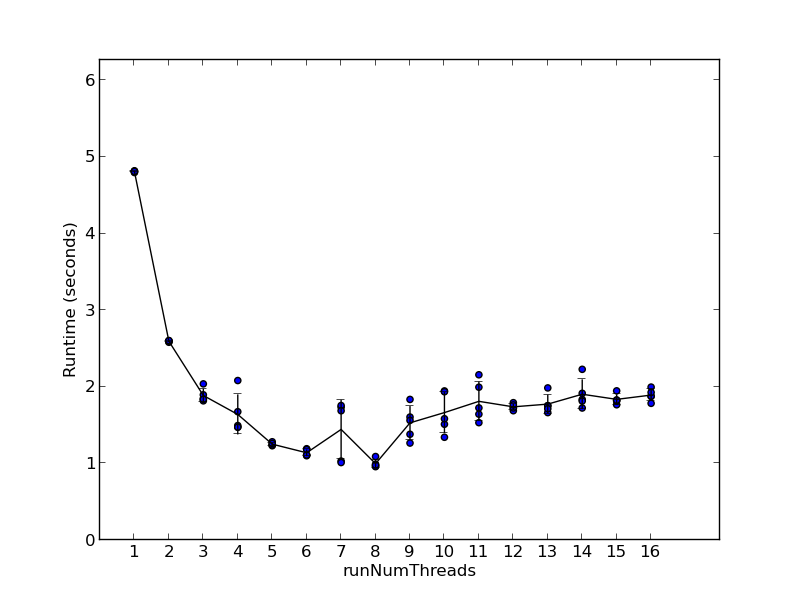
\includegraphics[scale=0.40]{{{images/threads-log3-catzilla.inf.ed.ac.uk-3-1}}}
    \end{centering}
  }
  \end{minipage}
  \begin{minipage}[t]{0.49\columnwidth}
  \subfloat[Throughput]{
    \begin{centering}
    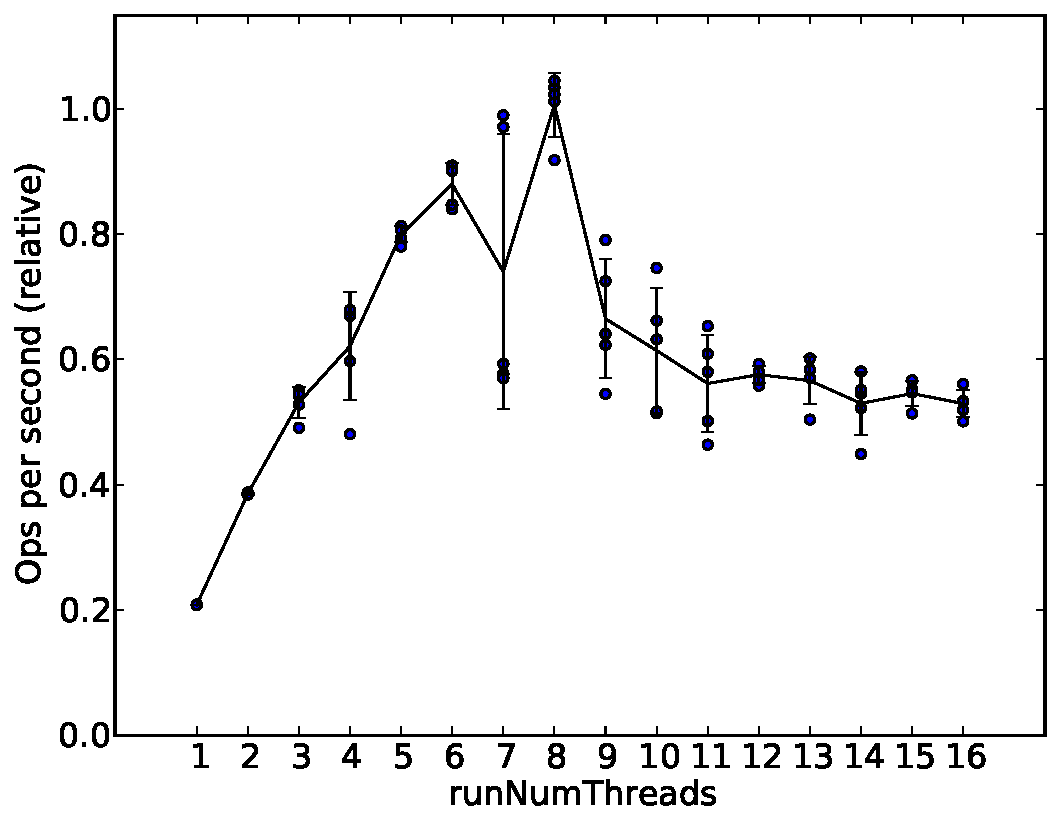
\includegraphics[scale=0.40]{{{images/threads-log3-catzilla.inf.ed.ac.uk-3-2}}}
    \end{centering}
  }
  \end{minipage}
  \caption{Runtime with 1 to 16 threads on Catzilla, Method 3, Logistics domain}
  \label{fig:thread-c3l}
  \end{figure}
  
  \section{Analysis}
  TODO
  
  \chapter {Method 4 - Single Global Queue}
  
  This method uses a single global queue of tasks, guarded by a mutual exclusion lock.
  
  \section {Implementation}
  
  The main thread adds a single empty explanation to the global queue, then spawns a worker thread for each hardware thread available. These threads all attempt to lock the queue and extract work from it. If they cannot lock the queue, they sleep until the lock becomes available. If they lock the queue and find it empty, they sleep for a fixed period of time, then try again. Once they complete the task, they lock the queue to put all the newly generated work on the queue, then resume trying to pull a task from the head of the queue.
  
  [TODO: code snippet]
  
  \section{Evaluation}
  
  \subsection{Batch Size Parameter}
  
  In order to estimate the best value for the batch size parameter, we again ran the implementation with 4 threads on the XPERIENCE domain, varying the batch size.
  
  \begin{figure}[!htbp]
  \begin{centering}
  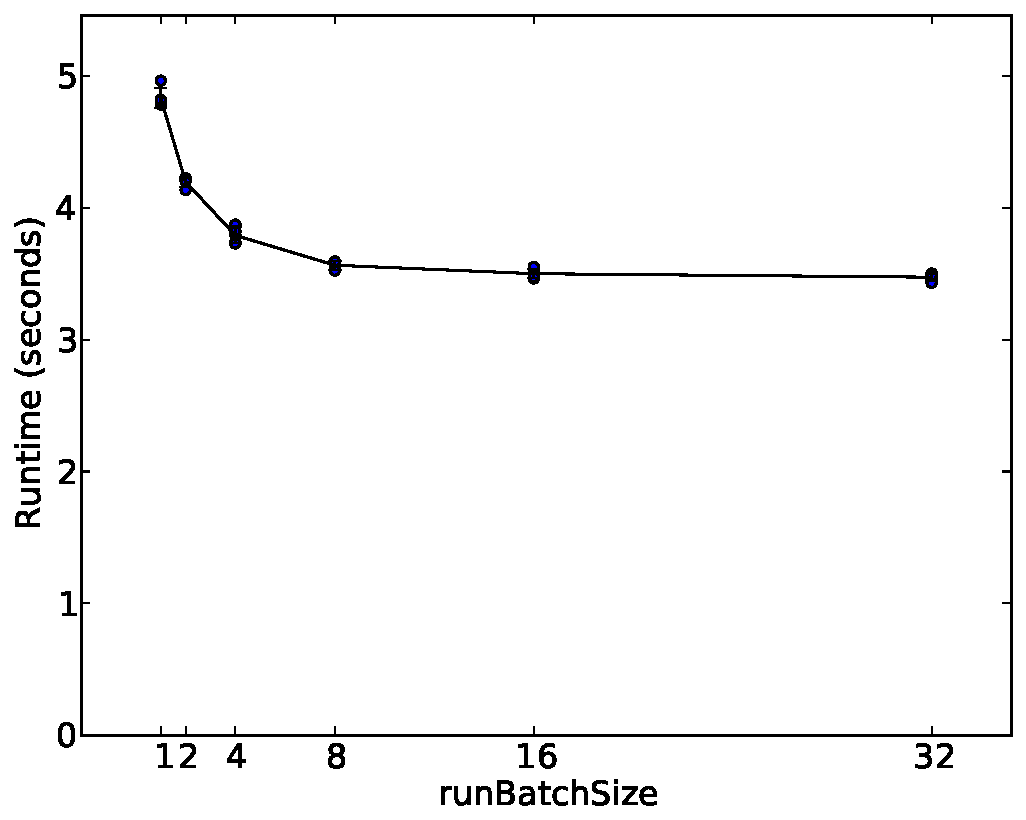
\includegraphics[width=0.8\textwidth]{images/batch-xper5-sherlock-4-1}
  \par\end{centering}
  \caption{Work-Stealing Runtime with varying batch size on Sherlock, XPERIENCE domain}
  \label{fig:batch-4}
  \end{figure}
  
  We can see in Figure~\ref{fig:batch-4} that the batch size parameter does have an effect on the runtime of this algorithm, suggesting that contention for the lock is worse with small tasks leading for more frequent insertions and removals on the global queue. In this test the runtime is similar from 8 explanations per batch upward, so all further tests were performed with a batch size of 8.
  
  \subsection{Thread Count}
  T\begin{figure}[!htbp]
  \centering{}
  \begin{minipage}[t]{0.49\columnwidth}
  \subfloat[Runtime]{
    \begin{centering}
    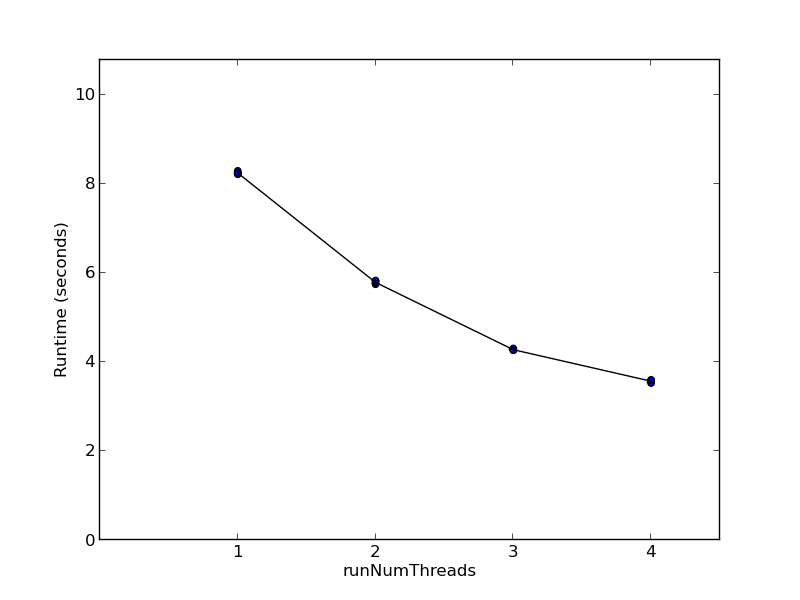
\includegraphics[scale=0.40]{{{images/threads-xper5-sherlock-4-1}}}
    \end{centering}
  }
  \end{minipage}
  \begin{minipage}[t]{0.49\columnwidth}
  \subfloat[Throughput]{
    \begin{centering}
    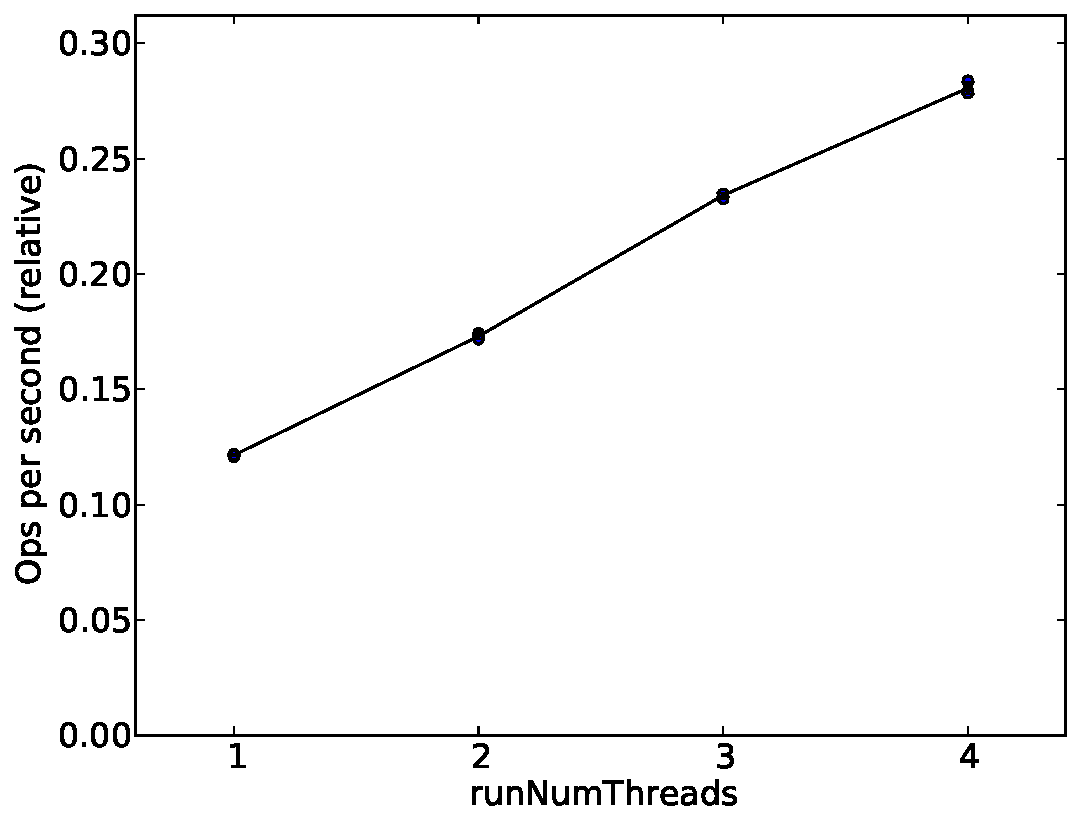
\includegraphics[scale=0.40]{{{images/threads-xper5-sherlock-4-2}}}
    \end{centering}
  }
  \end{minipage}
  \caption{Runtime with 1 to 4 threads on Sherlock, Method 4, XPERIENCE domain}
  \label{fig:thread-s4x}
  \end{figure}
  
  \begin{figure}[!htbp]
  \centering{}
  \begin{minipage}[t]{0.49\columnwidth}
  \subfloat[Runtime]{
    \begin{centering}
    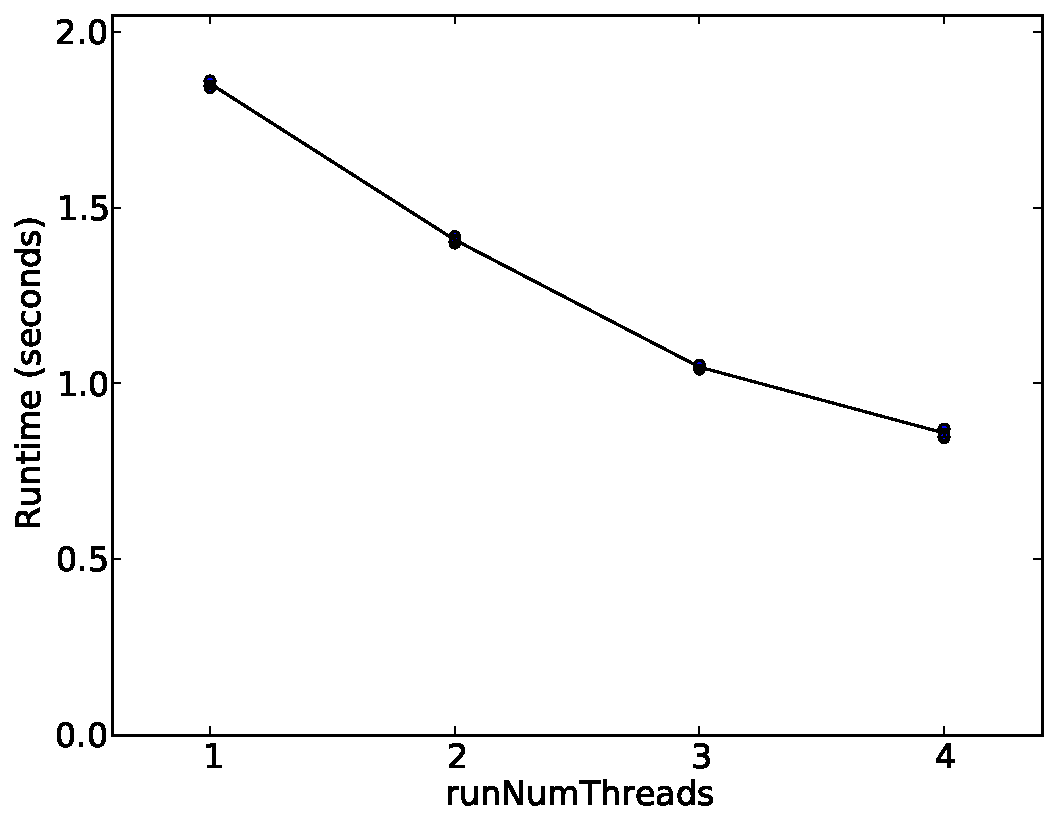
\includegraphics[scale=0.40]{{{images/threads-log3-sherlock-4-1}}}
    \end{centering}
  }
  \end{minipage}
  \begin{minipage}[t]{0.49\columnwidth}
  \subfloat[Throughput]{
    \begin{centering}
    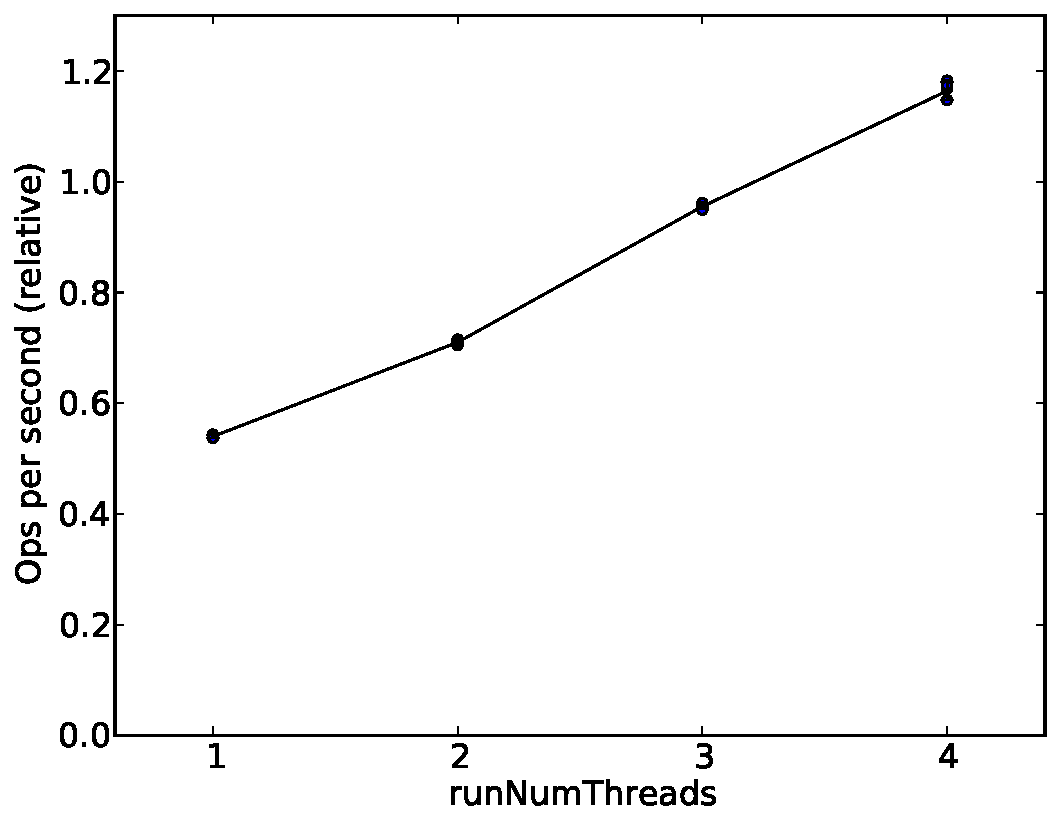
\includegraphics[scale=0.40]{{{images/threads-log3-sherlock-4-2}}}
    \end{centering}
  }
  \end{minipage}
  \caption{Runtime with 1 to 4 threads on Sherlock, Method 4, Logistics domain}
  \label{fig:thread-s4l}
  \end{figure}
  
  \begin{figure}[!htbp]
  \centering{}
  \begin{minipage}[t]{0.49\columnwidth}
  \subfloat[Runtime]{
    \begin{centering}
    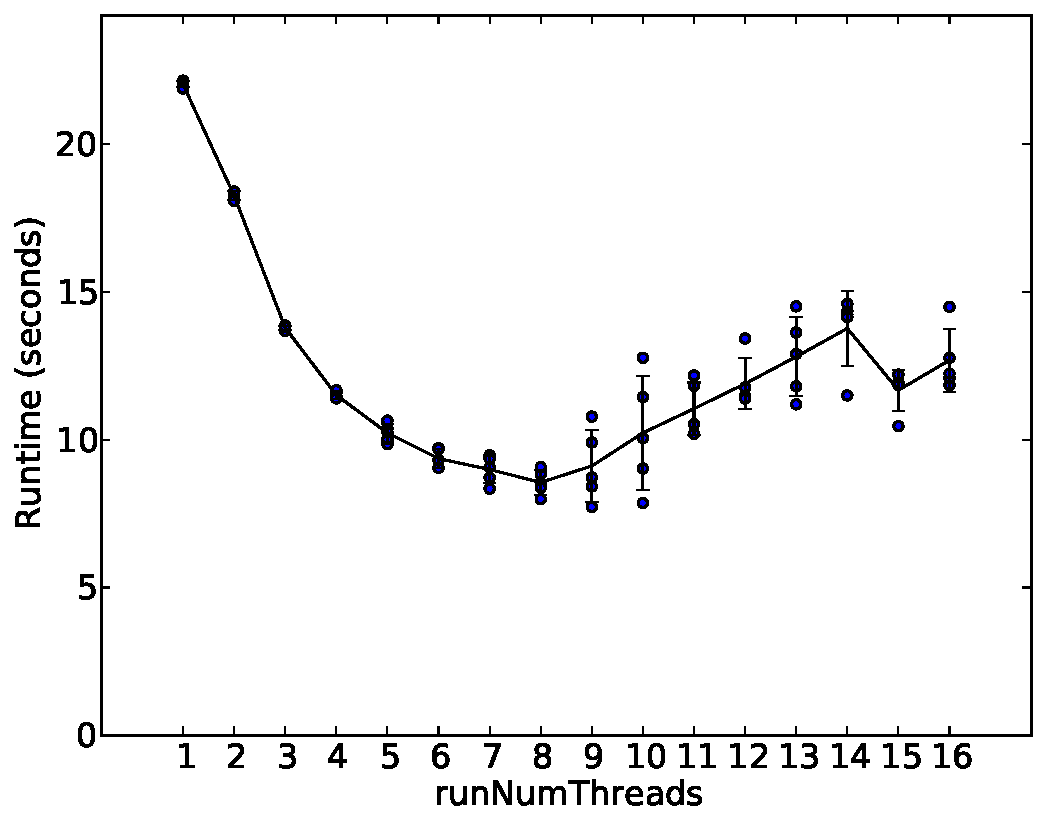
\includegraphics[scale=0.40]{{{images/threads-xper5-catzilla.inf.ed.ac.uk-4-1}}}
    \end{centering}
  }
  \end{minipage}
  \begin{minipage}[t]{0.49\columnwidth}
  \subfloat[Throughput]{
    \begin{centering}
    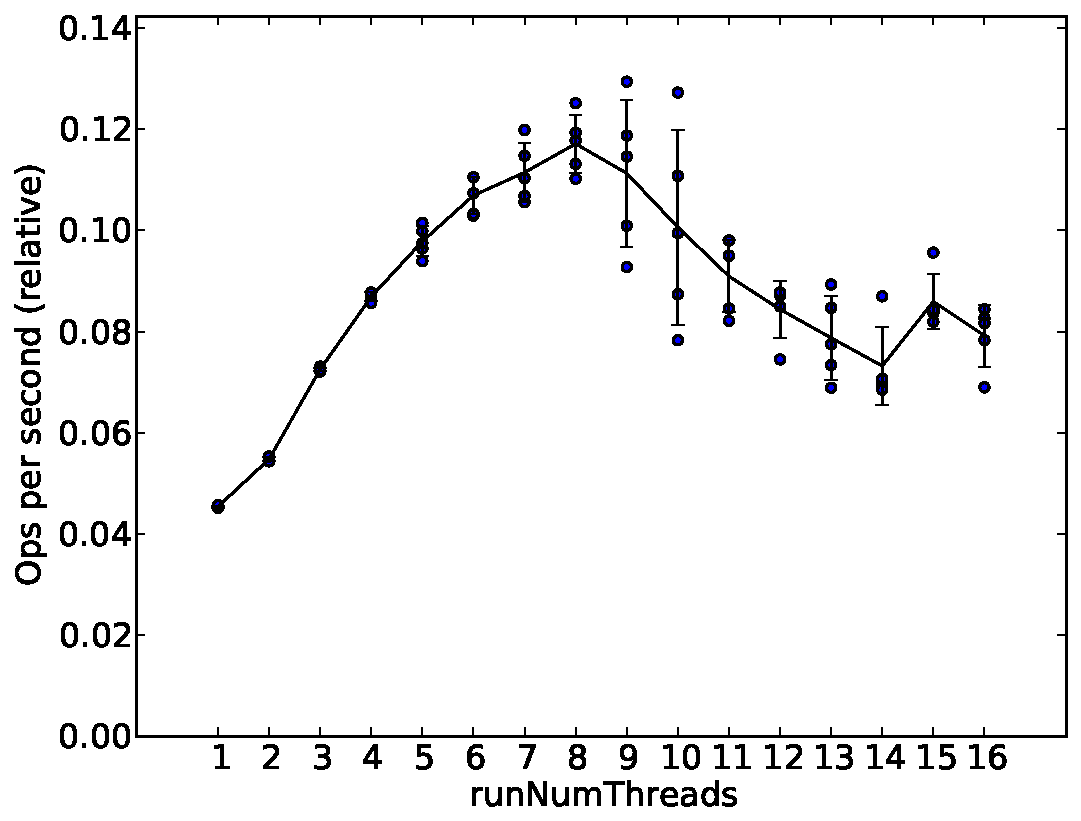
\includegraphics[scale=0.40]{{{images/threads-xper5-catzilla.inf.ed.ac.uk-4-2}}}
    \end{centering}
  }
  \end{minipage}
  \caption{Runtime with 1 to 16 threads on Catzilla, Method 4, XPERIENCE domain}
  \label{fig:thread-c4x}
  \end{figure}
  
  \begin{figure}[!htbp]
  \centering{}
  \begin{minipage}[t]{0.49\columnwidth}
  \subfloat[Runtime]{
    \begin{centering}
    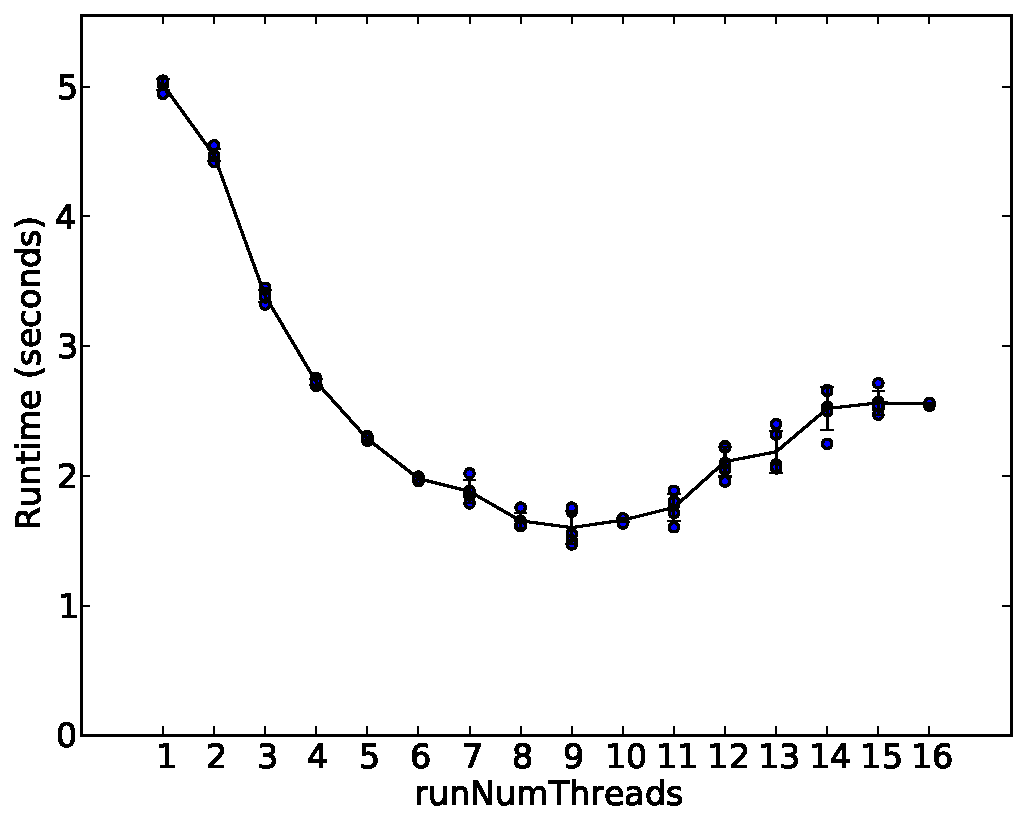
\includegraphics[scale=0.40]{{{images/threads-log3-catzilla.inf.ed.ac.uk-4-1}}}
    \end{centering}
  }
  \end{minipage}
  \begin{minipage}[t]{0.49\columnwidth}
  \subfloat[Throughput]{
    \begin{centering}
    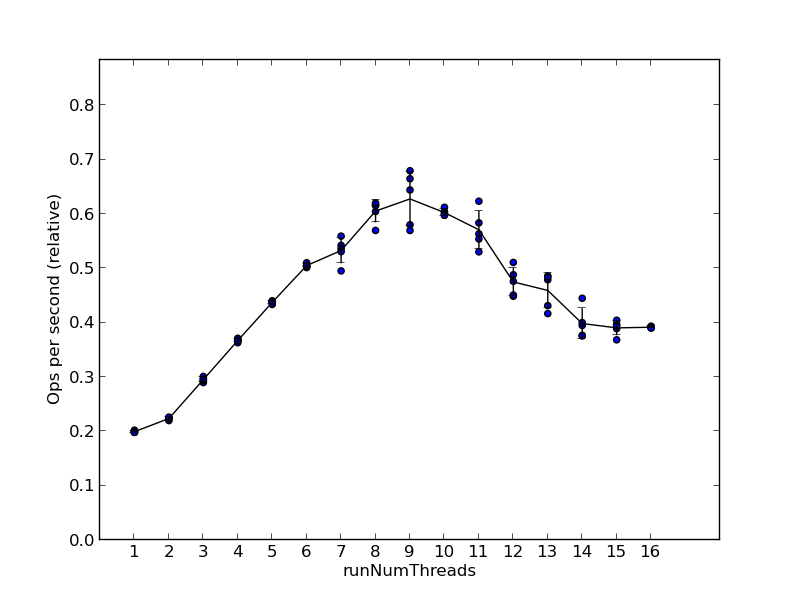
\includegraphics[scale=0.40]{{{images/threads-log3-catzilla.inf.ed.ac.uk-4-2}}}
    \end{centering}
  }
  \end{minipage}
  \caption{Runtime with 1 to 16 threads on Catzilla, Method 4, Logistics domain}
  \label{fig:thread-c4l}
  \end{figure}
  
  \section{Analysis}
  TODO
  
  % \chapter{Design}

TODO
   
  % \chapter{Implementation}

\section{Choice of Language \& Technologies}

The first big implementation decision that was made was the choice of language
that was used to create the system. Before the beginning of term I had made
a proof-of-concept of the system using \emph{C}. I found that the pace of
development was too slow and difficult to make rapid progress. As such
I decided to go in a different direction.

In order to have a shallower learning curve I decided to use a language that
I was familiar with: \emph{Ruby}. I've used Ruby extensively before on many
personal and coursework projects. Besides the experience benefits withe the
language there are other fantastic things about it.

\begin{description}

  \item[Community \& Existing Libraries] \hfill

    There is an extensive preexisting Ruby community that is extremely helpful
    and active. The advantage of this in my case is that there are already many
    libraries for the boilerplate or lower level code that I will be using.
    Importantly it already had bindings for \ac{FUSE} so writing the filesystem
    component of the project could be started immediately.

  \item[Testing Culture] \hfill

    Due to the dynamic nature of the language such as the ability to redefine
    and augment existing classes at runtime it is possible for the programmer
    to create situations where code performs differently based on possible
    hidden factors that have occurred before the execution. This is an
    extremely powerful and useful tool but it must be handled in the correct
    way to eliminate the risk of error. One of the ways that has evolved to
    cope with this is a strong testing culture that is mandated by the
    community for almost all Ruby projects.

    There are numerous libraries that make testing Ruby code quick and easy
    such as \emph{RSpec}. Additionally, large \emph{Ruby} frameworks such as
    \emph{Ruby on Rails} have been developed from the ground up to allow for
    simple and native testing. This culture inspires an Agile attitude to
    refactoring and improving code quality.

  \item[Portability] \hfill

    \emph{Ruby} runs on a number of different operating systems and platforms.
    This factored into my choice as I did not want the available systems that
    the project could run on to be limited by the language. In the end, it was
    \ac{FUSE} (see section \ref{ssec:filesystem}) that was the limiting
    portability factor.

\end{description}

\subsection{Filesystem}
\label{ssec:filesystem}

\ac{FUSE} is often used when creating a filesystem for a custom purpose. It
allows the developer to write code that responds to certain callbacks after it
has been mounted on the existing filesystem at a certain directory. For
example, when a directory is requested \ac{FUSE} will ask the developer's code
what objects are present in that directory by supplying it the argument of
a path. \ac{FUSE} then queries each of these objects to find out if they are
a file or a folder and if there are any permissions that would not allow them
to be shown. These results are then displayed to the user in their file
explorer as if they were actually entities on disk. This has a major advantage
over regular filesystem development which is extremely difficult and requires
extensive knowledge of the kernel to complete.

Other callbacks are provided for the developer to use. The file contents, size,
when files are deleted, or written to are all callbacks that are detected by
\ac{FUSE} and then passed on to the developer's code with the relevant
arguments to the action (e.g. the path being deleted or the text that has been
written to a file).

\subsection{Query GUI}

As discussed above, it isn't simply possible for a query interface to be added
to the filesystem and so a separate but integrated application needed to be
made in order to satisfy this requirement. I elected to use Java and Swing to
complete this task as it is a mature and stable \ac{GUI} toolkit that is
supported on a wide range of operating systems. It is more important that this
application is more portable than the filesystem itself because it would be
feasibly possible to mount the filesystem above over \ac{NFS} and only have
this application on the clients computer to interact with it.

To build the application that allows the user to query the database a GUI
toolkit was needed. Unfortunately \emph{Ruby} is not a suitable language for
this task as it does not have any mature, powerful, and platform-independent
GUI toolkits.

In order to develop this stage I decided to use \emph{Java} and the
\emph{Swing} interface library. This decision was made for two main reasons.

\begin{description}
  \item[Portability] \hfill

    The language that was used for this application must be able to run on any
    platform that the filesystem was used. One of the main advantages of using
    \emph{Java} in any project is that the same code and sometimes even the
    same executable can be run on multiple platforms and systems. This is
    thanks to the ``Write once, run everywhere.'' design
    consideration\footnote{In reality this is more likely to be ``Write once,
    debug everywhere.''}.

  \item[Familiarity] \hfill

    Due to previous projects, jobs, and coursework I am very familiar with the
    \emph{Java} language. Choosing a language that I know well will result in
    better quality code along with a faster development time.

  \item[GUI Toolkit] \hfill

    The \emph{Swing} GUI toolkit for \emph{Java} has its problems (verbosity,
    ugliness). However, even with these problems considered it is still the
    best fit for the application. Selecting \emph{Java} reduced the choices for
    possible interface libraries and due to the fantastic documentation,
    extensibility and customisability then \emph{Swing} was the sensible
    choice.

\end{description}

\section{Development}

\subsection{Filesystem}

The first stage of development was to create the filesystem on which all of the
other projects are based. As mentioned above, over summer I had created
a proof-of-concept system that allowed the user to view a read-only filesystem
representing a database. This was written in \emph{C} and used the native
\emph{FUSE} bindings. Not being satisfied with the development time and
complexities of the language and library I switched to using \emph{Ruby} and
the \emph{FuseFS} library.

The \emph{FuseFS} library works by ``mounting'' a class in a certain directory.
This class is required to implement certain methods (though due to the lack of
type-safety in \emph{Ruby} this can all fall apart at runtime). These methods
are then called when the user interacts with the filesystem whereupon the
return value from the called function is interpreted by the library and shown
in the filesystem. An example of the ``Hello World'' filesystem is shown in
figure~\ref{fig:fusefs}. This filesystem contains a single file called
\texttt{hello.txt} which when read has the contents \texttt{Hello, World!}.

\begin{figure}
% \begin{minted}[linenos]{ruby}
\begin{lstlisting}
class HelloDir
  def contents(path)
    ['hello.txt']
  end

  def file?(path)
    path == '/hello.txt'
  end

  def read_file(path)
    "Hello, World!\n"
  end

  def size(path)
    read_file(path).size
  end
end
%\end{minted}
\end{lstlisting}
  \caption{A Sample \emph{FuseFS} filesystem.}
  \label{fig:fusefs}
\end{figure}

Using this library I created the filesystem that allowed the user to manipulate
databases. Each table was represented as a directory in the filesystem and
inside were files representing the records in those tables. Each of these were
formatted as \texttt{csv} files for ease of development and portability between
many different spreadsheet editors.

It was noticed that there was no way to select only certain columns to display
in these CSV files rather than just displaying all of them. A new directory was
added inside the table that allowed a user to move columns (represented again
as files) between two folders denoting the used and unused columns. Initially
it was planned that the user would be able to drag the file between the two
directories in order to change this. However, it was found that when using
\ac{FUSE} a file move only looks like a file deletion and a new file write with
no link between them. To overcome this the method which the user changes the
selected columns was changed to use the delete action. This is not ideal and
should be later changed to a more suitable action.

Similar to the \texttt{/proc} filesystem which my project gained much of its
inspiration I added files that could be read to find out information about the
database. For example, this includes the name, list of tables, path, and string
encoding. This allows users to easily find out information by only reading
a file instead of interrogating the database.

\subsubsection{Filesystem DSL Library}

The more I developed this system the slower it became to add new functionality
as the code became more complex. During the Christmas break I decided to write
a new library for creating these filesystem definitions. I decided to start out
with the ``dream library'' by writing down (in \emph{Ruby}) how \emph{I} would
like to build the filesystem. I have included the example I originally wrote in
figure~\ref{fig:skra}. This new \ac{DSL} library is called
\emph{Skra}\footnote{Skr\'{a} is Icelandic for ``file'' or ``directory''.}.

The example below creates a filesystem that is mounted at \texttt{/mount/point}
and contains a directory called \texttt{hello} which has read and write
permissions. Inside this directory are two files: one named \texttt{path} which
contains its own path and the other is called \texttt{time} which when read
will return the current time.

Using this library allowed me to develop the remainder of the project far more
quickly and easily. The library itself was an interesting program to write due
to its implementation as a DSL.

\begin{figure}
%\begin{minted}[linenos]{ruby}
\begin{lstlisting}
Filesystem.new "/mount/point" do
  directory "hello", :perms => [:r, :w] do
    file "path" do |path|
      # File contains its own path.
      path
    end

    file "time" do |path|
      # Shows the current time.
      Time.now.to_s
    end
  end
end
%\end{minted}
\end{lstlisting}
  \caption{An example \emph{Skra} layout.}
  \label{fig:skra}
\end{figure}

\subsection{Query Language}

You may have noticed above that I have not mentioned how the database is
queried. This is due to the query problem that was mentioned earlier in
section~\ref{sec:queryproblem}. The solution which was decided on above was to
create a two-tiered system for querying. Firstly, a language is created that
allows even complex queries to be written sequentially and out of order. This
allows more advanced users to use this directly when querying. Secondly, an
application is created that allows users who are not familiar with databases to
invisibly create this language before using the same process as the more
advanced users to query the database. This section deals with the creation of
this intermediate language.

At the time this was planned to only be a very small part of a larger project
and as such spending a large portion of time creating a whole new language with
its own grammar, parser, and semantics was not a wise time investment. In order
to gain all of these language building blocks for ``free'' \emph{Ruby} was
again used. The \emph{Ruby} language has often been used as the base of other
\acp{DSL} such as the build tool
\emph{Rake}\footnote{http://rake.rubyforge.org/} or the testing framework
\emph{RSpec}\footnote{http://rspec.info/}. Both of these tools have a syntax
that while being completely executable is able to be expressive and simple.

Using this same trait of \emph{Ruby} in the \ac{DSL} allowed the creation of
a query language that did not resemble its parent language while using it as
a strong foundation. By using \emph{Ruby} the fantastic library \emph{ARel}
library\footnote{\url{https://github.com/rails/arel}} could also be used in
order to generate the \ac{SQL} from relational algebra. \emph{ARel} is
a powerful and mature piece of software (it powers the \ac{ORM} in the popular
web framework \emph{Ruby on Rails}). However, it is not designed to be directly
used in the manner required for this project and as such additional changes
were required in order to make it suitable for the \ac{DSL}.

Various additions were made to allow for a clean interface between the two
sides of the system. New functions that improved the ease-of-use and script
like qualities of the language were added (e.g. The \texttt{Table} function
which removed the ugly overhead required to define a new table for use in
\emph{ARel}). A command line interface was added to the system to complete its
functionality. The entire system was named \emph{Squeal} as it was a Pig Latin
for \ac{SQL}. An example query is shown in figure~\ref{fig:squeal}.

\begin{figure}
%\begin{minted}[linenos]{ruby}
\begin{lstlisting}
users = Table :users
grades = Table :grades

# Define predicates separately
predicate = users[:name].eq("Chris Brown")

# Simply Sequential
user_grades = join(users, grades, :id, :user_id)
user_where = where(user_grades, predicate)
user_window = limit(user_where, 1)

# Useful Chaining
user_order = user_window.order(grades[:mark])

Output select(user_grades, grades[:course], grades[:mark])
%\end{minted}
\end{lstlisting}
  \caption{A Squeal script for finding the course and mark for the lowest
  grade on record.}
  \label{fig:squeal}
\end{figure}

\subsection{Query GUI}

In order to generate this language a \ac{GUI} needs to be created that allows
users to draw the graph representation of their query. This program can then be
used by users of all experience levels. The advantage of using relational
algebra for our intermediate language is that is is composeable and therefore
a graph based interface can be used to create these queries.

As discussed above, \emph{Swing} and \emph{Java} were used in order to create
the interface. The most challenging component of this was creating a new user
interface element for the graph. This component was completely custom and it
was built with reuse in mind. This component can be embedded in other
applications if the developer wishes for a pre-built solution for building
these queries.

The user interface is extremely minimal. The only significant element in the
window is the graph creation component mentioned above. All of the user
interaction with the program is done by using the right-click menu of this
component. When a user has finished creating their query they are able to
easily save this file to the filesystem where it is executed.

The operation of the program is relatively simple. Users right click on the
canvas and place nodes corresponding to the different operators that can be
performed by the query. After a node is placed the user is prompted to enter
the attributes of the node (such as the number of records to limit or the
predicate of a filter node). The user is then able to drag connectors between
these nodes in order to create the final query.

An example of a query is shown in figure~\ref{fig:bacon}. This would generate
the Squeal script that was shown before in figure~\ref{fig:squeal}.

\begin{figure}
  \centering
  \includegraphics[width=0.9\textwidth]{images/bacon}
  \caption{Example GUI Query}
  \label{fig:bacon}
\end{figure}

  
  % Analysis: results and their critical analysis should be reported, whether the results conform to expectations or otherwise and how they compare with other related work.
  
  \chapter{Evaluation}

TODO describe histogram of number of generated explanations for each existing one, and how this informs design choices

TODO here compare the different approaches, have graphs with results from all algorithms

TODO describe choice of metrics (or do this earlier?)

TODO describe the domains used (or do this earlier?)

TODO discuss hyperthreading and how it affects scaling of performance with number of threads (mention this in background too?)

TODO compare the speedup we get to a perfect $T_1$ to $T_\infty$ speedup

\subsection{XPERIENCE Domain}
TODO

\begin{figure}[!htbp]
\begin{centering}
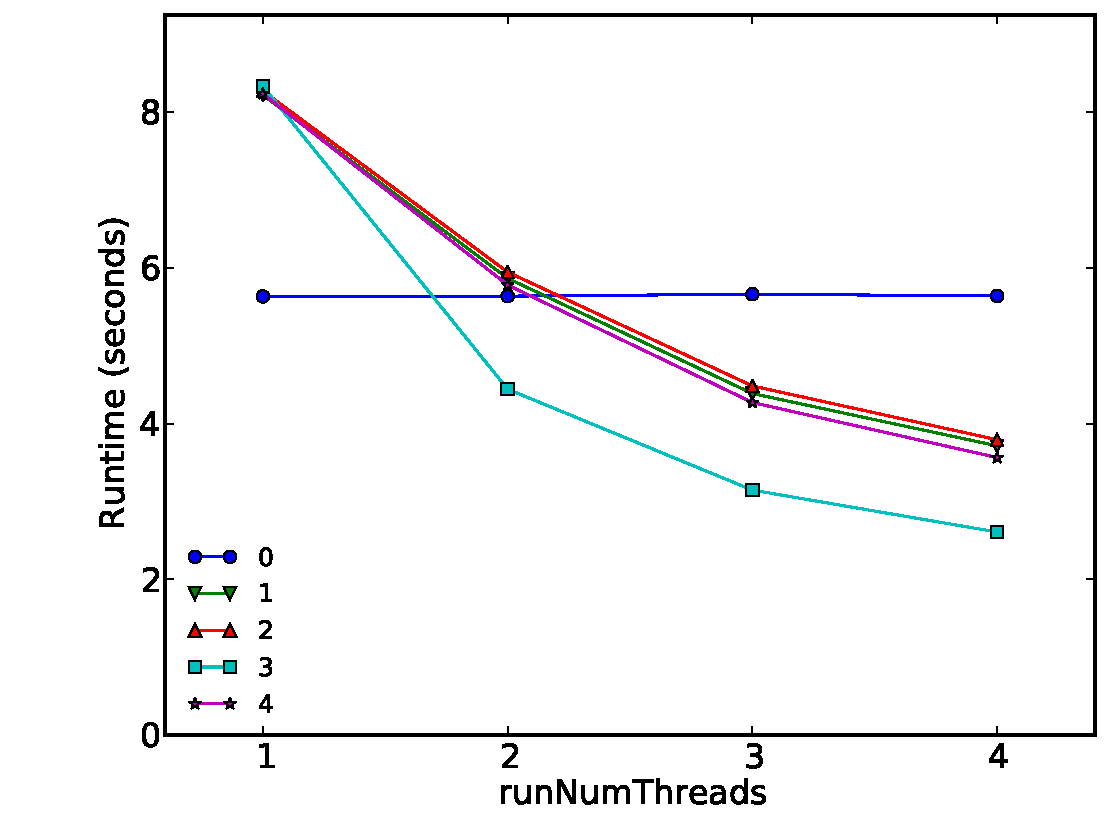
\includegraphics[width=0.8\textwidth]{images/threads-xper5-sherlock-all-1}
\par\end{centering}
\caption{Work-Stealing Runtime with 1 to 4 threads on Sherlock, All Methods, XPERIENCE domain}
% \label{}
\end{figure}

\subsection{Logistics Domain}
TODO

\begin{figure}[!htbp]
\begin{centering}
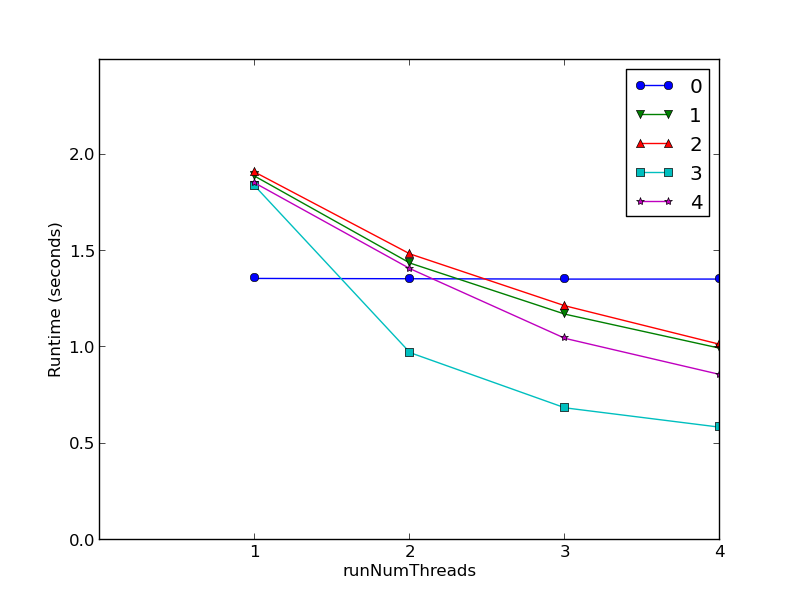
\includegraphics[width=0.8\textwidth]{images/threads-log3-sherlock-all-1}
\par\end{centering}
\caption{Work-Stealing Runtime with 1 to 4 threads on Sherlock, All Methods, Logistics domain}
% \label{}
\end{figure}
  % Conclusion:
  \chapter{Conclusion}

Due to the widespread usage of database systems throughout the modern world it
is essential that there are usable interfaces for using and exploring the data
inside them. These interfaces must be generic and fit many kinds of data in
order to be reused cheaply and without waste for many different databases. By
opening up these databases to a wider audience we enable users with expertise
in fields that are able to use this data without requiring that they learn the
intricacies of databases.

In this project I have designed and built what I believe to be one possible
solution to this problem. We allow far more users to explore the contained data
by presenting the data contained in the records and tables of a database to the
user in the familiar interface paradigm of files and directories.

Being able to explore and edit the data easily is just the first step in
improving the accessibility to all users. The next step is allowing the user to
perform more complex queries of this information. To accomplish this I have
built a new application that allows users to create queries using a graph based
interface. Users unequivocally preferred using this interface compared to using
\ac{SQL} even if they knew the latter technology well.

I believe that the tools above, when combined, form a system that is a solution
to the original problem of general database accessibility and visualisation for
users of all skill levels.


  % Appendix
  \appendix

  % \chapter{Evaluation}

\section{Tasks}
\label{sec:tasks}

\begin{enumerate}
\item What is the matriculation number of the oldest student?
\item What is the first name of the student with the matriculation number \texttt{0824586}?
\item What is the highest grade that the student with \texttt{id=6} achieved?
\item What is the name of the student with the lowest grade overall?
\item Which students take the course \texttt{Maths 101}?
\end{enumerate}

\section{Schema}
\label{sec:schema}

% not in the repo? \includegraphics[width=1.0\textwidth]{images/schema.pdf}

\section{Results}

\subsection{User 1}

\subsubsection{Information}

\begin{tabular}{|l|l|}
	\hline
	\textbf{Prior Database Experience} & First Year Course \\
	\hline
\end{tabular}

\subsubsection{Task Timing}

\begin{tabular}{|l|l|c|c|c|c|c|}
	\hline
	\multicolumn{2}{|r|}{\textbf{Task}} & \textbf{1} & \textbf{2} & \textbf{3} & \textbf{4} & \textbf{5} \\
	\hline
	\multirow{2}{*}{Time (s) [Correct]} & SQL   & -   & -   & -   & -   & -   \\
	                                            & Graph & 145 [YES] & 148 [YES] & 291 [YES] & 250 [YES] & 205 [NO] \\
	\hline
\end{tabular}

\subsubsection{Notes and Difficulties}

\begin{itemize}

	\item
	User looked for a help document.

	\item
	User did not understand the difference between \textbf{select} and \textbf{filter}.

	\item
	User was confused by difference between the operators \textbf{equal} and \textbf{matches}.

	\item
	User attempted to move the nodes once they were placed.

\end{itemize}

\subsection{User 2}

\subsubsection{Information}

\begin{tabular}{|l|l|}
	\hline
	\textbf{Prior Database Experience} & First Year Course \\
	\hline
\end{tabular}

\subsubsection{Task Timing}

\begin{tabular}{|l|l|c|c|c|c|c|}
	\hline
	\multicolumn{2}{|r|}{\textbf{Task}} & \textbf{1} & \textbf{2} & \textbf{3} & \textbf{4} & \textbf{5} \\
	\hline
	\multirow{2}{*}{Time (s) [Correct]} & SQL   & 48 [NO]  & 19 [YES] & 35 [NO]  & -   & -   \\
	                                       & Graph & 46 [YES] & 49 [YES] & 106 [NO] & 69 [YES] & 170 [NO] \\
	\hline
\end{tabular}

\subsubsection{Notes and Difficulties}

\begin{itemize}

	\item
	User did not understand the difference between \textbf{select} and \textbf{filter}.

\end{itemize}

\subsection{User 3}

\subsubsection{Information}

\begin{tabular}{|l|l|}
	\hline
	\textbf{Prior Database Experience} & First, Third, and Fourth Year Courses \\
	\hline
\end{tabular}

\subsubsection{Task Timing}

\begin{tabular}{|l|l|c|c|c|c|c|}
	\hline
	\multicolumn{2}{|r|}{\textbf{Task}} & \textbf{1} & \textbf{2} & \textbf{3} & \textbf{4} & \textbf{5} \\
	\hline
	\multirow{2}{*}{Time (s) [Correct]} & SQL   & 90 [NO]  & 23 [YES] & 70 [YES] & 129 [NO]  & 73 [YES]   \\
	                                    & Graph & 70 [YES] & 42 [YES] & 167 [YES] & 113 [YES] & 125 [YES] \\
	\hline
\end{tabular}

\subsubsection{Notes and Difficulties}

\begin{itemize}

	\item
	User had no issues.

\end{itemize}

\subsection{User 4}

\subsubsection{Information}

\begin{tabular}{|l|l|}
	\hline
	\textbf{Prior Database Experience} & First Year Course \\
	\hline
\end{tabular}

\subsubsection{Task Timing}

\begin{tabular}{|l|l|c|c|c|c|c|}
	\hline
	\multicolumn{2}{|r|}{\textbf{Task}} & \textbf{1} & \textbf{2} & \textbf{3} & \textbf{4} & \textbf{5} \\
	\hline
	\multirow{2}{*}{Time (s) [Correct]} & SQL   & 99 [YES] & 21 [YES] & 73 [YES] & 130 [YES] & 65  [YES] \\
	                                    & Graph & 89 [YES] & 35 [YES] & 93 [YES] & 137 [YES] & 163 [NO]  \\
	\hline
\end{tabular}

\subsubsection{Notes and Difficulties}

\begin{itemize}

	\item
	User attempted to delete a node.

	\item
	User complained that right click was difficult.

	\item
	User attempted to move a node that was already placed.

	\item
	User was confused with how to use the join node.

	\item
	User was confused about how to use the output of 2 joins.

\end{itemize}

  % Bibliography
  \bibliography{sections/misc/z_bib.tex}{}
  \bibliographystyle{unsrt}
\end{document}
